\chapter{前馈神经网络}
\label{chap:feedforward-networks}

第~\ref{chap:neural-network-overview}章用异或说明了隐藏表示的作用：两个非线性单元就能把原始坐标中无法线性分开的样本变成可分的表示。但那组权重是手工给出的，真实数据有成千上万个参数，不可能手工填写。本章要把这个演示变成一套可以实际运行的方法，需要依次回答三个问题：网络内部的计算究竟怎样组织（结构问题）？这些参数怎样从数据中自动得到（学习问题）？又凭什么相信在训练数据上表现好的网络，对没见过的新样本仍然可靠（泛化问题）？

本章以最基础、也最常用的一类网络——层状、全连接的前馈神经网络——为对象，把前章的函数复合落实为可计算、可求导的具体模型。本章的推进路线是：先规定一次预测中数据如何逐层流动，以及不同任务末端应该输出什么、用什么损失打分（\ref{sec:ffn-structure}节）；再解决训练的两个前置环节——参数的初始取值和反向传播这一核心求导算法，并说明实际框架如何自动完成求导（\ref{sec:ffn-learning}节）；然后把模型接口扩展到设备型号、词这样的高维离散类别输入，即Embedding（\ref{sec:ffn-extensions}节）；最后从理论上严格区分三件容易混淆的事：网络\emph{能不能}表达目标函数、优化算法\emph{能不能}找到好参数、找到的参数在新数据上\emph{风险有多大}（\ref{sec:ffn-theory}节）。阅读本章需要用到向量与矩阵运算、偏导数与链式法则，以及前几卷的损失、梯度下降等概念。

\section{网络结构}
\label{sec:ffn-structure}

本节先把“一个网络”精确地写成可以逐行实现的计算。所谓\emph{前馈}，规定的只是计算依赖的方向：同一次前向计算中，信息从输入出发逐层流向输出，后面的结果不会通过任何有向环再流回上游去影响本次计算。至于每层内部具体如何连接、一层放多少个单元，则是可以另行选择的设计。我们采用最简单也最稠密的一种安排——全连接的逐层结构，并把一次预测拆成三个环节反复观察：先对输入做\emph{加权组合}，再作\emph{非线性响应}形成新特征，最后由一个与任务相配的\emph{输出层}给出预测。

\subsection{神经元}
\label{sec:ffn-neuron}

网络的最小构件是一个人工神经元。它做的事可以用一句话概括：读取若干个数值，判断这些数值整体上支持还是反对它所关注的某种模式，再给出一个响应强度。这种“判断”不是硬规则，而是通过加权求和实现的。设单元的输入为$\bm{u}\in\mathbb{R}^{m}$，权重为$\bm{w}\in\mathbb{R}^{m}$，偏置为$b\in\mathbb{R}$，则
\begin{equation}
  z=\bm{w}^{\top}\bm{u}+b,
  \qquad h=\sigma(z)\text{。}
  \label{eq:ffn-unit}
\end{equation}
先看加权和$z=\bm{w}^{\top}\bm{u}+b$。内积$\bm{w}^{\top}\bm{u}$可以从几何上理解：当$\bm{u}$与权重向量$\bm{w}$方向接近时内积较大、方向相反时较小甚至为负，因此权重$\bm{w}$相当于刻划了单元“期待看到的输入方向”——输入越符合这个方向，加权和越高。每个权重决定对应输入以多大强度、正向还是负向影响结果。偏置$b$则是在不看任何输入时就存在的一个基准分，它改变单元开始响应的位置：没有偏置时，ReLU单元正负区域的分界线$\bm{w}^{\top}\bm{u}=0$被迫经过原点；加入偏置后这条分界可以平移到任意位置，单元的判定因此不再受“原点必须在边界上”的限制。

加权和之后还要经过激活函数$\sigma$。这里的$z$称为\term{预激活值}（pre-activation），即非线性变换之前的原始加权结果；$h$是非线性变换后的单元输出。为什么不能直接输出$z$？因为如果每个单元都只做加权求和，上一章已经证明，多层堆叠仍会合并成一次线性变换；正是$\sigma$的非线性让多层网络有了超出线性模型的能力，各种$\sigma$的选择见\ref{sec:ffn-activations}节。

单个单元只能产生一个新特征。让许多个这样的单元并排，各自用不同的权重读取同一组输入，就能同时产生一组不同视角的新坐标，这就是\term{全连接层}（fully connected layer）：下一层的每个单元都与上一层的每个单元相连。把一个单元的权重作为矩阵的一行，整层计算就可以用一次矩阵乘法完成，而不必逐个单元循环。沿用前章的列向量约定，设网络有$L$个隐藏层，输入为$\bm{x}\in\mathbb{R}^{d}$，令$d_0=d$、$\bm{h}^{(0)}=\bm{x}$，各隐藏层依次计算
\begin{equation}
  \begin{aligned}
    \bm{z}^{(\ell)}
      &=\bm{W}_\ell\bm{h}^{(\ell-1)}+\bm{b}_\ell,\\
    \bm{h}^{(\ell)}&=\sigma_\ell\!\left(\bm{z}^{(\ell)}\right),
    \qquad \ell=1,\ldots,L\text{。}
  \end{aligned}
  \label{eq:ffn-hidden-layers}
\end{equation}
其中$\bm{W}_\ell\in\mathbb{R}^{d_\ell\times d_{\ell-1}}$、$\bm{b}_\ell\in\mathbb{R}^{d_\ell}$，$\bm{z}^{(\ell)}$和$\bm{h}^{(\ell)}$都属于$\mathbb{R}^{d_\ell}$，$\sigma_\ell$逐坐标作用。上标$\ell$表示层的位置，不是幂，也不是参数更新的迭代步。

隐藏层之后还需一个与任务相配的输出层。记原始输出为$\bm{a}\in\mathbb{R}^{q}$、$d_{L+1}=q$，完整模型写为
\begin{equation}
  \begin{aligned}
    \bm{a}&=\bm{W}_{L+1}\bm{h}^{(L)}+\bm{b}_{L+1},\\
    \widehat{\bm{y}}&=g(\bm{a})\text{。}
  \end{aligned}
  \label{eq:ffn-output-map}
\end{equation}
矩阵$\bm{W}_{L+1}\in\mathbb{R}^{q\times d_L}$和向量$\bm{b}_{L+1}\in\mathbb{R}^{q}$参与学习，输出变换$g$由任务决定。$g$可以是恒等映射，也可以把得分转换为概率。用$\bm{\theta}\in\mathbb{R}^{p}$收集全部权重与偏置，模型记为$\bm{f}_{\bm{\theta}}(\bm{x})=\widehat{\bm{y}}$；标量输出时写$f_{\bm{\theta}}$。

图~\ref{fig:ffn-architecture}展示了这种分层依赖。输入层只提供数据，不计算一组新的可学习参数；隐藏层的每个坐标都是一次式\eqref{eq:ffn-unit}的计算。这就是前章引入的多层感知机：具有一个或多个全连接隐藏层、用非线性变换构造表示的前馈网络。这里的MLP采用可供梯度计算的非线性激活，区别于早期感知机作硬判定的阈值响应。

\begin{figure*}[htb]
  \centering
  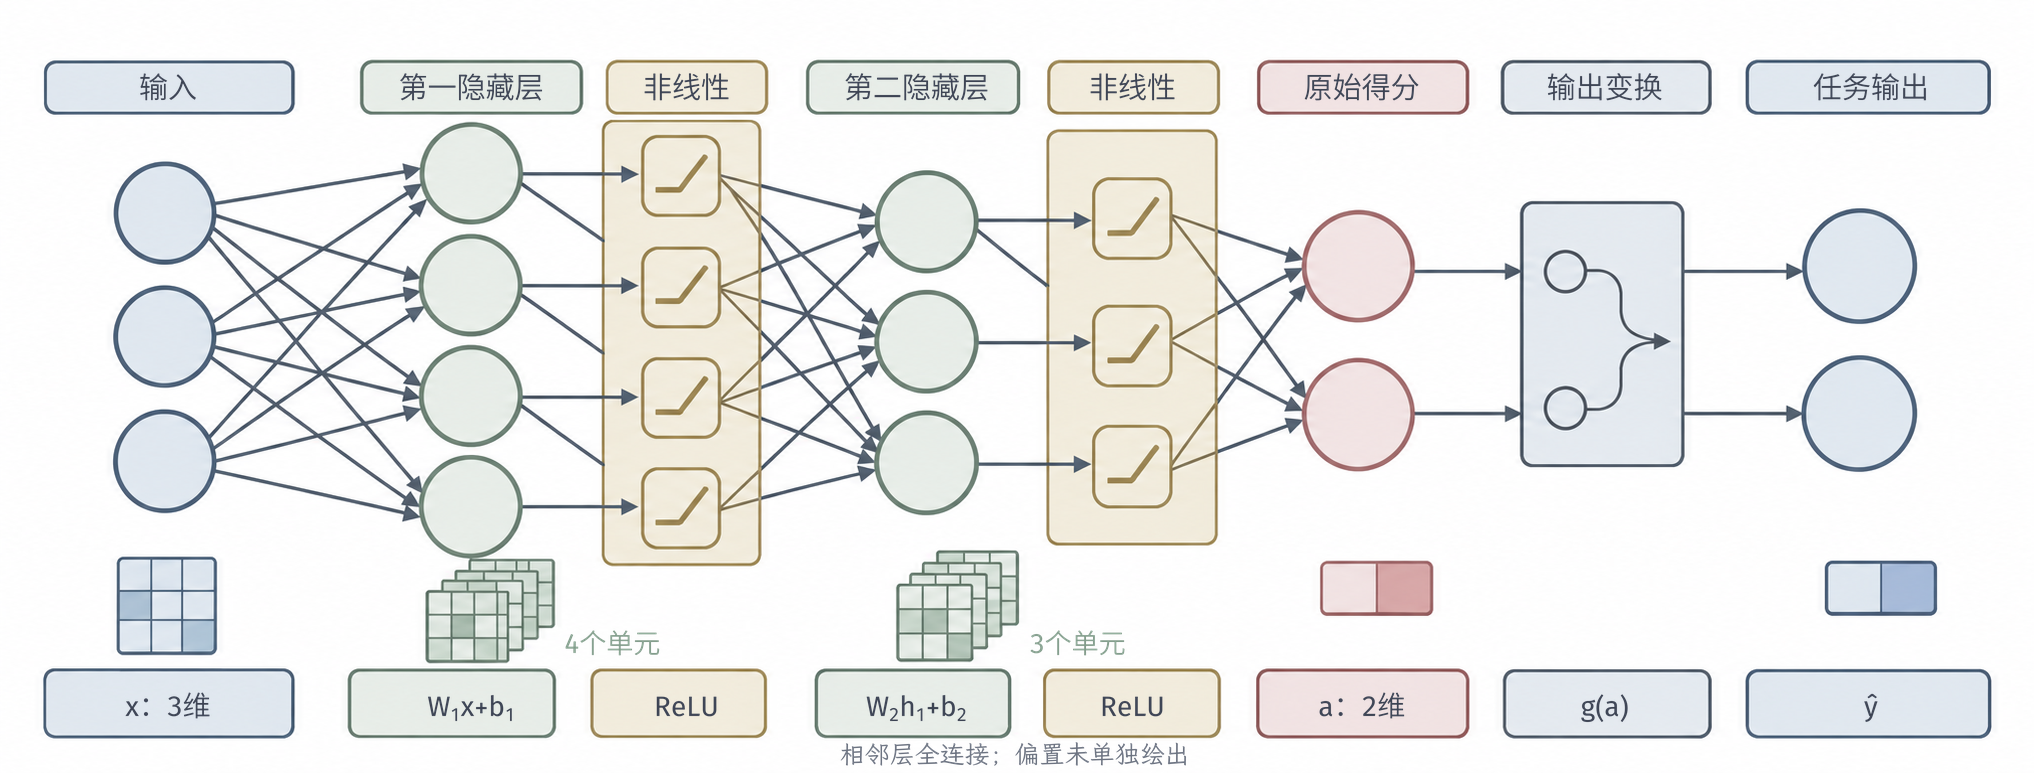
\includegraphics[width=169.000mm]{figures/05-neural-network-models/00-shared/generated/ffn-architecture/figure.png}
  \caption{两个隐藏层的全连接前馈网络。左侧单元提供输入$\bm{x}$，中间两层计算隐藏表示，右侧单元产生原始得分$\bm{a}$，之后再使用任务规定的输出变换$g$。细线表示可学习的连接，层间箭头标明前向计算方向；每个目标单元还具有一个未画出的偏置。图中层宽依次为$3,4,3,2$，只是结构示例。}
  \label{fig:ffn-architecture}
\end{figure*}

对没有参数共享的上述网络，参数总数为
\begin{equation}
  p=\sum_{\ell=1}^{L+1}d_\ell(d_{\ell-1}+1)\text{。}
  \label{eq:ffn-parameter-count}
\end{equation}
这个式子可以这样核对：第$\ell$层有$d_\ell$个单元，每个单元读取前一层$d_{\ell-1}$个输出，需要$d_{\ell-1}$个输入权重，再加上$1$个偏置，于是每个单元有$d_{\ell-1}+1$个参数，整层为$d_\ell(d_{\ell-1}+1)$，各层相加即为总数。若输入维度为$100$，两个隐藏层宽度均为$64$，输出维度为$1$，参数量为$64\times101+64\times65+65=10689$。这个数字主要被$100\times64$的第一层占据，说明输入编码的维度和层宽会直接决定模型规模；这也是为什么面对高维输入（如图像的几十万像素），后面章节会用卷积等结构来避免全连接带来的参数爆炸。忽略激活和偏置的较小开销，一次单样本前向计算的乘加量与$\sum_\ell d_\ell d_{\ell-1}$同阶，因为计算量主要花在每层的矩阵乘法上。需要提醒的是，参数量和计算量只描述\emph{规模}：同样数量的参数能表达哪些关系由连接方式与激活函数决定，而预测是否可靠还需要训练数据与泛化分析来回答。

本文把$L$称为隐藏层数，把$d_\ell$称为第$\ell$层宽度。文献中的\term{深度}（depth）有时包含输出层，有时只计隐藏层，两种计数相差一个输出层，因此深度比较需要采用同一口径。跨层连接只要不构成有向环，也可以保持前馈性质；本章的逐层推导采用普通串联结构。

\subsection{激活函数}
\label{sec:ffn-activations}

上一章已经证明，连续叠加仿射层仍然只是一次仿射变换，因此隐藏层必须使用非线性激活。但“非线性”只是一个最低要求，实践中激活函数的种类很多，初学时容易被一长串名字淹没。理解它们的关键是抓住一个统一的视角：\emph{激活函数决定一个预激活值$z$如何变成单元输出，而不同的“形状”会在三个方面产生不同后果}——它能表达什么样的输入—输出关系、反向传播时梯度能否顺利通过、输出落在什么数值范围。

为了让下面的介绍有线索可循，可以先按“形状”把常见函数分成几类。最朴素的基准是恒等函数（什么都不做）和阶跃函数（只给0/1硬判定）。在需要概率等有界输出时，会用到把任意实数压进有限区间的\emph{双侧饱和函数}，如Sigmoid和Tanh；它们在输入很大或很小时输出几乎不再变化，这种“压平”会带来梯度变小的问题。为缓解这一问题，\emph{整流函数}（以ReLU为代表）选择只截断负值、对正值原样放行，由此衍生出一批带泄漏、带上界的变体；\emph{指数型函数}让负值平滑地趋向一个有限下界而非硬截断；\emph{自门控函数}（Swish、GELU等）则让输入乘以一个随自身连续变化的“保留比例”，在正负区域之间平滑过渡。最后，Maxout和Softmax比较特殊：它们不逐个坐标独立作用，而是\emph{联合处理一组}预激活值。

需要事先说明三点阅读约定。其一，带可学习参数的函数（如PReLU、Swish）曲线形状会随训练改变，图中画出的具体参数值只是比较时的一个条件，不是固定结论。其二，随机型函数（如RReLU）在训练和预测两个阶段采用的规则可能不同。其三，除特别说明外，下面都把输入记为标量$z$、输出记为$\sigma(z)$，因为绝大多数激活是逐坐标独立作用的；理解了一个坐标上的形状，整层只是把同样的规则并行施加到每个坐标。

\subsubsection{恒等与阶跃}
\label{sec:ffn-activation-baselines}

若需要保留任意实数输出，可以使用\term{恒等函数}（identity function）；若只需要一个硬的二值判定，可以使用\term{阶跃函数}（step function）。两者分别为
\begin{equation}
  \operatorname{Identity}(z)=z,
  \qquad
  H(z)=\begin{cases}0,&z<0,\\1,&z\geq0\text{。}\end{cases}
  \label{eq:ffn-identity-step}
\end{equation}
恒等函数的导数为$1$，常用于回归输出或无需额外激活的投影；全部隐藏层都用恒等函数时，多层串联仍是仿射映射。阶跃函数适合表达阈值决策，但除阈值处不可微之外，在其余位置导数都为$0$，普通反向传播无法据此学习阈值单元的输入参数。预测时作硬判定与训练时使用连续可导替代，是两种不同用途。

\begin{figure*}[htb]
  \centering
  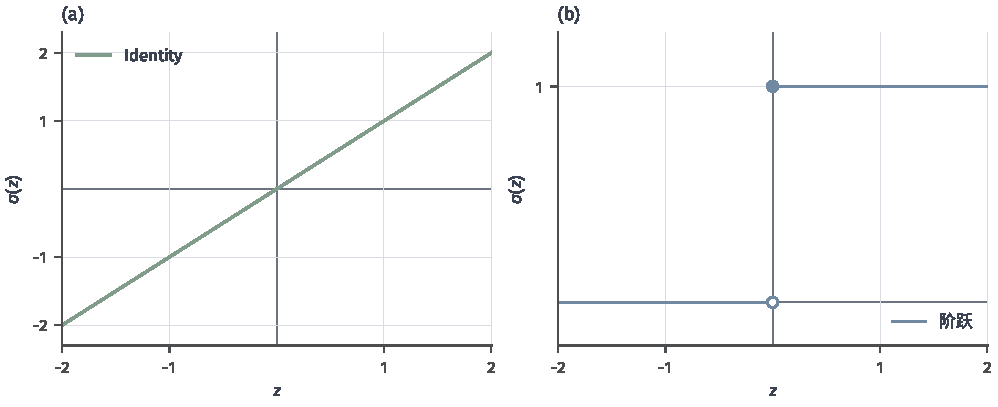
\includegraphics[width=159.059mm]{figures/05-neural-network-models/00-shared/matplotlib/ffn-activation-basics/figure.pdf}
  \caption{恒等函数与阶跃函数的比较。左图保留输入，斜率恒为$1$；右图按零阈值输出$0$或$1$，空心点和实心点区分$z=0$两侧的端点约定。横轴为预激活值$z$，纵轴为输出；阶跃图中的跳跃不能通过普通局部导数传递学习信号。}
  \label{fig:ffn-activation-basics}
\end{figure*}

\subsubsection{双侧饱和函数}
\label{sec:ffn-activation-saturating}

当一个单元需要产生概率、控制系数或有界状态时，把任意实数压到有限区间是直接的选择。\term{Logistic函数}产生$(0,1)$内的响应，实践中常直接称为Sigmoid；\term{双曲正切函数}（hyperbolic tangent, Tanh）产生$(-1,1)$内的响应。Sigmoid也可泛指具有S形曲线的一类函数，这里用$s$专门表示Logistic函数：
\begin{equation}
  \begin{aligned}
    s(z)&=\frac{1}{1+\exp(-z)},
    &s'(z)&=s(z)(1-s(z)),\\
    \tanh(z)&=\frac{\exp(z)-\exp(-z)}{\exp(z)+\exp(-z)},
    &\tanh'(z)&=1-\tanh^2(z)\text{。}
  \end{aligned}
  \label{eq:ffn-saturating-activations}
\end{equation}
当$|z|$很大时，输出接近两端的极限，导数趋近于零。这种\term{饱和}（saturation）意味着输入继续变化，输出却几乎不变。Sigmoid导数至多为$1/4$；Tanh在原点的导数为$1$，并满足$\tanh(z)=2s(2z)-1$。Tanh关于原点对称，可以产生正负响应，但只有对称输入分布等条件才能进一步推出输出均值为零。

Sigmoid适合二分类概率、多标签概率和取值在$(0,1)$的控制门。当损失与事件标签构成概率模型时，这一响应才作为相应事件的概率；用在隐藏层时，它只是有界特征值。Tanh适合需要正负有界状态的模块，例如后续循环网络中的候选状态。两者用于许多层连续串联时，饱和区的小导数可能参与梯度衰减；传播中的权重矩阵同时可以放大或缩小信号，完整梯度尺度由沿途的两种作用共同决定。

若希望避免指数运算，可以用分段线性函数近似上述有界响应。\term{硬Sigmoid}（hard sigmoid，也称Hard-Logistic）和\term{硬Tanh}（hard tanh）将线性段之外的值截到边界：
\begin{equation}
  \begin{aligned}
    \operatorname{HardSigmoid}(z)
      &=\min\{1,\max\{0,\tfrac14z+\tfrac12\}\},\\
    \operatorname{HardTanh}(z)&=\min\{1,\max\{-1,z\}\}\text{。}
  \end{aligned}
  \label{eq:ffn-hard-saturating-activations}
\end{equation}
本节的HardSigmoid在$(-2,2)$内斜率为$1/4$，区间外为$0$；HardTanh在$(-1,1)$内斜率为$1$，区间外为$0$，其负端输出是$-1$。分段边界处的导数需要约定。HardSigmoid的线性段并没有唯一标准，一些实现采用$z/6+1/2$并在$\pm3$处截断；不同斜率与截断点会改变响应及导数，移植模型需要采用与原实现相同的定义\scite{pytorchHardsigmoid}

两种硬近似可用于受计算资源限制的门控或范围约束，代价是拐点不可微，截断区内还会出现严格为零的梯度。\term{Softsign函数}提供另一种有界响应，用绝对值而非指数控制幅度：
\begin{equation}
  \operatorname{Softsign}(z)=\frac{z}{1+|z|},
  \qquad
  \operatorname{Softsign}'(z)=\frac{1}{(1+|z|)^2}\text{。}
  \label{eq:ffn-softsign}
\end{equation}
它的值域也是$(-1,1)$，一阶导数连续，尾部导数以多项式速度趋零。它可用于需要有界正负响应的隐藏层或状态映射；与Tanh相比，它的尾部导数衰减更慢，具体输入处的梯度大小仍由各自导数值决定。

\begin{figure*}[htb]
  \centering
  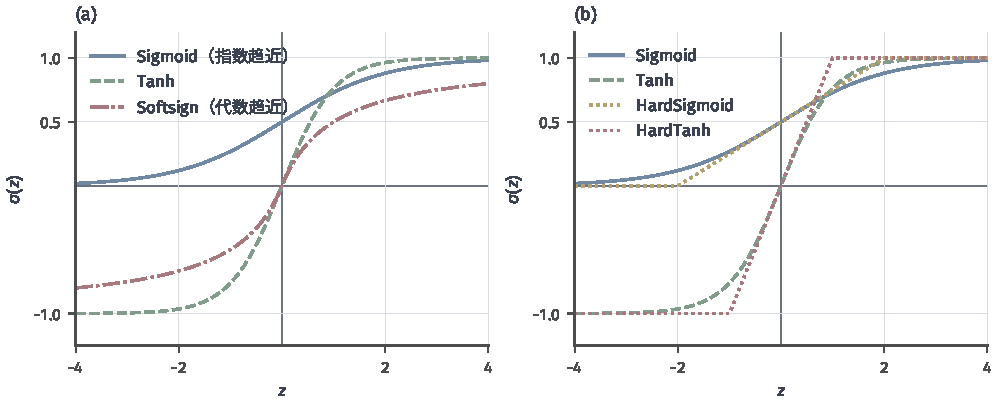
\includegraphics[width=159.059mm]{figures/05-neural-network-models/00-shared/matplotlib/ffn-activations/figure.pdf}
  \caption{双侧饱和激活函数。左图比较Logistic／Sigmoid、Tanh与Softsign；Softsign采用长虚线，以便在黑白打印中仍能与Sigmoid区分，图例同时指出前者按代数速度、后者按指数速度趋近渐近值。右图将HardSigmoid和HardTanh与对应平滑函数比较。HardSigmoid采用式\eqref{eq:ffn-hard-saturating-activations}中的斜率$1/4$及截断点$\pm2$。}
  \label{fig:ffn-activations}
\end{figure*}

\subsubsection{整流函数及其变体}
\label{sec:ffn-activation-rectifiers}

ReLU采用前章的$\rho(z)=\max\{0,z\}$，正半轴斜率为$1$，负半轴输出和导数都为$0$。它只需一次比较和一次取值，不涉及指数运算，并且能够产生严格为零的激活（即一批单元在某个样本上完全关闭），因而是全连接或卷积隐藏层最常用的基础选择。

ReLU的简洁也带来一个特有的训练现象。设想某个单元：对当前所有训练样本，它的加权和$z$都落在负半轴，于是输出恒为$0$。由于负半轴导数为$0$，损失对这个单元输入权重的梯度也是$0$，梯度下降不会再修改这些权重；权重不变，$z$的分布也不变，该单元就可能一直停在关闭状态，称为“单元失活”或“死亡ReLU”。需要澄清两点：失活是\emph{当前参数与当前数据共同}造成的结果，并非单元本身损坏；它也未必永久。如果更上游的表示在后续训练中发生变化，使某些样本的$z$回到正半轴，这个单元仍可能被重新激活。尽管如此，大面积失活意味着一部分参数事实上退出了学习，这正是后面引入“负半轴保留斜率”等变体的直接原因。

让负半轴保留非零斜率，可以避免该区域完全阻断局部梯度。\term{带泄漏的ReLU}（leaky ReLU）使用固定$0<\alpha<1$，\term{参数化ReLU}（parametric ReLU, PReLU）则把负半轴斜率作为待学习参数：
\begin{equation}
  \begin{aligned}
    \operatorname{LeakyReLU}(z)
      &=\max\{0,z\}+\alpha\min\{0,z\},\\
    \operatorname{PReLU}_j(z)
      &=\max\{0,z\}+\alpha_j\min\{0,z\}\text{。}
  \end{aligned}
  \label{eq:ffn-leaky-prelu}
\end{equation}
PReLU的$\alpha_j$可以按单元、通道设置，也可以在一层内共享；若不另加约束，它并不天然位于$(0,1)$。给定上游梯度，斜率参数的局部求导规则是$\partial\operatorname{PReLU}_j(z)/\partial\alpha_j=\min\{0,z\}$，共享斜率时要累加各使用位置的贡献。PReLU增加的参数量取决于共享方式，通常每个单元、通道或层只增加一个斜率参数\scite{he2015rectifiers}

Leaky ReLU适合希望保留负响应且不增加待学习参数的隐藏层，PReLU适合允许数据调整负响应强度的模块。\term{随机化带泄漏ReLU}（randomized leaky ReLU, RReLU）沿用同一分段形式，但训练时从预先规定的区间$[l,u]$均匀采样负斜率$\alpha$，其中$0<l<u<1$，预测时通常采用$(l+u)/2$。每次采样产生一条不同曲线，使同一负输入在训练中受到不同缩放。预测采用确定斜率；这种训练扰动对误差的作用需要在相应任务上评价\scite{xu2015rectified}

如果部署还要求限制正响应，可以使用\term{ReLU6函数}，即
\begin{equation}
  \operatorname{ReLU6}(z)=\min\{6,\max\{0,z\}\}\text{。}
  \label{eq:ffn-relu6}
\end{equation}
它在$(0,6)$内保留斜率$1$，在两侧导数为$0$，常与移动端模型及有限数值范围的设计联系在一起。MobileNetV2使用了这类有界整流响应，但其线性瓶颈层还刻意省略非线性，说明激活要按层的职责选择\scite{sandler2018mobilenetv2}相对于ReLU，新增上界让较大的正输入也进入零导数区，有限范围与梯度传递因此形成取舍。

\begin{figure*}[htb]
  \centering
  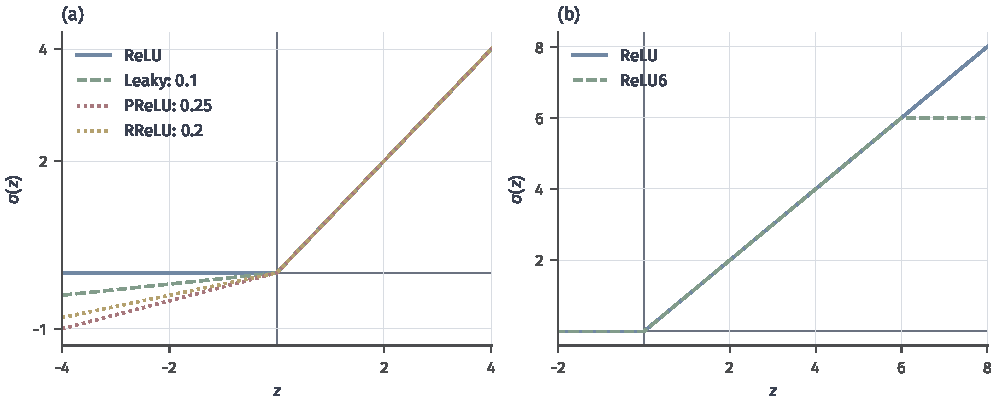
\includegraphics[width=159.059mm]{figures/05-neural-network-models/00-shared/matplotlib/ffn-activation-rectifiers/figure.pdf}
  \caption{整流函数与负斜率变体。左图固定Leaky ReLU的$\alpha=0.1$、PReLU的$\alpha_j=0.25$，并以$\alpha=0.2$画出RReLU训练阶段的一种可能曲线；三者的形状差异来自斜率选择，PReLU与RReLU的区别主要在参数取得方式。右图比较ReLU与ReLU6，展示$z>6$时的截断。两图横轴范围不同。}
  \label{fig:ffn-activation-rectifiers}
\end{figure*}

有界函数与整流函数的差异集中在表~\ref{tab:ffn-activation-bounded}中。Sigmoid、Tanh和Softsign限制两端幅度，ReLU只截断负半轴，ReLU6还限制正端；这种范围差异会直接改变哪些输入能够传递梯度。

\begin{table*}[htb]
  \centering
  \small
  \begin{tabularx}{\linewidth}{@{}l l X X@{}}
    \toprule
    函数 & 输出范围 & 导数与参数特点 & 适用场景及主要边界 \\
    \midrule
    Identity & $\mathbb{R}$ & 导数为$1$ & 回归输出、线性投影；不增加非线性 \\
    阶跃 & $\{0,1\}$ & 非阈值处导数为$0$ & 硬判定；不能直接靠普通反向传播训练 \\
    Sigmoid & $(0,1)$ & 两端导数趋零 & 二分类、多标签、控制门 \\
    Tanh & $(-1,1)$ & 两端导数趋零 & 有界正负状态；深层饱和需关注 \\
    HardSigmoid & $[0,1]$ & 截断区导数为$0$ & 简单门控；需核对斜率与截断点 \\
    HardTanh & $[-1,1]$ & 截断区导数为$0$ & 有界状态；拐点与严格零梯度 \\
    Softsign & $(-1,1)$ & 一阶连续，尾部导数趋零 & 有界正负表示；尾部衰减方式不同 \\
    ReLU & $[0,+\infty)$ & 负半轴为$0$，正半轴为$1$ & 全连接、卷积隐藏层；可能失活 \\
    Leaky ReLU & $\mathbb{R}$ & 固定正负斜率 & 保留负梯度；斜率需设定 \\
    PReLU & 依赖$\alpha_j$ & 负斜率参与学习 & 学习响应形状；需说明参数共享方式 \\
    RReLU & $\mathbb{R}$ & 训练时随机负斜率 & 隐藏层训练扰动；预测规则不同 \\
    ReLU6 & $[0,6]$ & 两侧截断，中间斜率为$1$ & 有限范围、移动端；正端也会饱和 \\
    \bottomrule
  \end{tabularx}
  \caption{有界响应与整流激活的比较。Leaky ReLU和RReLU的范围按正负斜率均为正且非零书写；PReLU若不限制斜率，其输出范围随参数改变。所有分段函数都需在不可微边界约定求导规则。}
  \label{tab:ffn-activation-bounded}
\end{table*}

即使都用于限制输出幅度，求导行为也可能不同。Tanh和HardTanh都提供有界正负响应；按解析定义，前者在有限输入下保留非零导数，后者在截断区的导数严格为零。选择范围约束时，还需判断训练中的预激活值是否经常落到这些区域。

\subsubsection{指数型与平滑整流函数}
\label{sec:ffn-activation-exponential}

固定负斜率让负输出无限下降，另一种做法是使负响应逐渐接近一个有限下界。\term{指数线性单元}（exponential linear unit, ELU）在正半轴保留输入，在负半轴使用指数曲线：
\begin{equation}
  \operatorname{ELU}_{\alpha}(z)=
  \begin{cases}
    z,&z>0,\\
    \alpha(\exp(z)-1),&z\leq0,
  \end{cases}
  \qquad \alpha>0\text{。}
  \label{eq:ffn-elu}
\end{equation}
负半轴导数为$\alpha\exp(z)$，对有限负输入非零，但在$z\to-\infty$时趋零；输出趋近$-\alpha$。ELU连续，只有$\alpha=1$时左右一阶导数才在原点一致，但原点左右的二阶导数不同。ELU可用于希望保留负值并控制负端幅度的隐藏层；负响应允许层输出向两侧分布，实际均值仍由输入分布和权重决定\scite{clevert2016elu}

仅知道单个单元怎样响应，还不足以判断多层堆叠后会发生什么，这里引入一个新的视角。固定网络参数，让输入随样本变化，则每个单元的输出都是一个随机变量：可以用均值描述它的“中心位置”、用方差描述它的“波动幅度”。当信号一层层传下去时，这两个统计量会被每层的权重和激活不断改变。如果每经过一层方差就放大一些，深层的输入数值会越来越大；如果方差不断缩小，数值又会被压向零。这两种趋势累积几十层后，都会让训练变得困难——前者容易使数值溢出或梯度过大，后者则使不同输入难以区分、梯度微弱。因此，一个自然的设计目标是：让每层输出的均值大致保持在零附近、方差大致保持在一附近，使信号在层间传播时尺度稳定。SELU正是为这一目标设计的激活函数。

\term{缩放指数线性单元}（scaled exponential linear unit, SELU）在ELU的基础上整体乘一个固定系数$\kappa$：
\begin{equation}
  \operatorname{SELU}(z)=\kappa
  \begin{cases}
    z,&z>0,\\
    \alpha(\exp(z)-1),&z\leq0,
  \end{cases}
  \label{eq:ffn-selu}
\end{equation}
其中常用常数为$\alpha\approx1.6733$、$\kappa\approx1.0507$。它用于\term{自归一化网络}（self-normalizing neural network），即在规定假设下让层间激活的均值与方差趋向受控范围的前馈网络。相应分析依赖输入与权重的统计条件；常配合输入标准化、权重方差为$1/\mathrm{fan\text{-}in}$的初始化，以及为保持统计量设计的AlphaDropout。这里fan-in是一个单元的输入连接数，初始化的具体说明见第~\ref{sec:ffn-initialization}节。自归一化结论依赖这套激活、初始化与丢弃规则共同满足统计假设，替换其中一项也会改变分析条件\scite{klambauer2017selu}

具体地，把一层输出的均值、方差记为$(\mu,\nu)$，下一层对应统计量记为$(\widetilde\mu,\widetilde\nu)$。原分析在输入坐标独立且同均值、同方差的设定下采用加权和的正态近似，这项近似本身也是后续结论的条件。当单元权重的和为零、平方和为一且偏置为零时，SELU中$\alpha$与$\kappa$的理论取值按统计映射把$(0,1)$仍送到$(0,1)$的要求选择。这就是零均值、单位方差的不动点含义。负端饱和与正端大于$1$的斜率分别提供限制幅度与放大响应的两种作用，常数选择让二者在统计目标附近形成平衡。在论文限定的输入统计量和权重范围内，偏离这一点的小扰动还会被后续映射缩小；训练中的任意权重和任意相关输入不自动满足这些条件。

训练时若要随机屏蔽活动值，还需避免屏蔽本身破坏上述统计目标。AlphaDropout（alpha dropout）把被屏蔽的值替换为SELU的负饱和值$\alpha_-=-\kappa\alpha$，再作仿射修正。以一个均值为零、方差为一的活动值$h$为例，令保留概率为$\pi\in(0,1]$，独立掩码$m_{\mathrm d}\sim\operatorname{Bernoulli}(\pi)$在保留时为$1$、替换时为$0$，替换后的值为
\[
  \widetilde h=m_{\mathrm d}h+(1-m_{\mathrm d})\alpha_-\text{。}
\]
保留部分的均值为零，替换部分恒为$\alpha_-$，所以$\mathbb E[\widetilde h]=(1-\pi)\alpha_-$。方差既包括保留时原有波动的贡献$\pi$，也包括保留与替换两种均值差异的贡献$\pi(1-\pi)\alpha_-^2$。因此可先减去新均值，再除以新标准差，得到
\[
  h_{\mathrm d}=
  \frac{\widetilde h-(1-\pi)\alpha_-}
       {\sqrt{\pi[1+(1-\pi)\alpha_-^2]}}\text{。}
\]
在上述均值、方差和掩码独立条件下，$h_{\mathrm d}$重新具有均值零与方差一。预测时关闭这项随机替换与配套修正，使用原有活动值。这个关系对活动值和掩码的分布计算，并不要求每个有限小批量的样本均值、样本方差都精确等于目标；它也没有单独保证整个训练过程收敛或预测风险降低。

如果目标是输出严格正值而又保持平滑，可以使用\term{Softplus函数}：
\begin{equation}
  \operatorname{Softplus}(z)=\log(1+\exp(z)),
  \qquad \operatorname{Softplus}'(z)=s(z)\text{。}
  \label{eq:ffn-softplus}
\end{equation}
它在正端接近$z$，在负端趋近$0$，但有限输入下输出严格大于$0$，不会产生ReLU式的精确零激活。Softplus可作为平滑隐藏激活，也适合将任意得分映射为正尺度、强度或方差参数；需要严格正下界时还可加上一个固定小常数。计算时使用$\max\{z,0\}+\log(1+\exp(-|z|))$可避免指数溢出。因此Softplus的用途由平滑性和正值约束决定；隐藏分类响应与正尺度输出采用它时，所要满足的条件不同。

\begin{figure}[htbp]
  \centering
  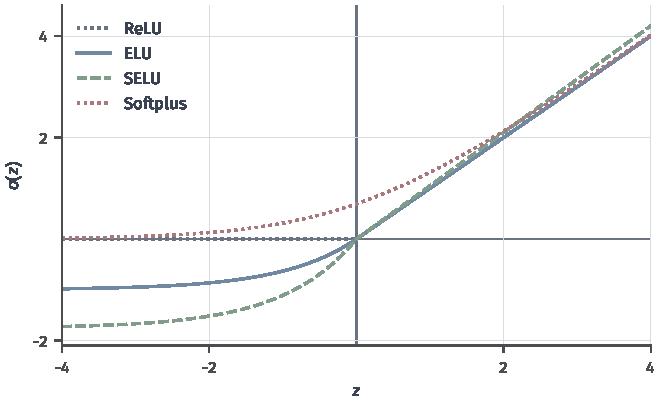
\includegraphics[width=105.412mm]{figures/05-neural-network-models/00-shared/matplotlib/ffn-activation-exponential/figure.pdf}
  \caption{ELU、SELU与Softplus的响应。ELU使用$\alpha=1$，SELU使用式\eqref{eq:ffn-selu}中的常数，ReLU作为共同参照。ELU与SELU允许负输出并在负端趋向有限下界；Softplus始终为正，且平滑地趋近正半轴上的线性响应。}
  \label{fig:ffn-activation-exponential}
\end{figure}

\subsubsection{自门控函数}
\label{sec:ffn-activation-self-gated}

ReLU根据输入的正负作硬切换，也可以让输入乘一个连续变化的系数。\term{Swish函数}使用输入自身计算保留系数：
\begin{equation}
  \operatorname{Swish}_{\beta}(z)=z s(\beta z),
  \qquad \beta\geq0\text{。}
  \label{eq:ffn-swish}
\end{equation}
$\beta$可以固定，也可以参与学习。$\beta=0$时函数为$z/2$；$\beta=1$时得到\term{Sigmoid加权线性单元}（sigmoid-weighted linear unit, SiLU）；当$\beta\to+\infty$时，对每个固定输入趋向ReLU。这里的极限只描述固定输入处的响应值；不同$\beta$还会改变各输入处的导数，从而改变训练过程\scite{ramachandran2017swish}

计算输入敏感度及可学习门参数的梯度，需要分别对输入与门参数求导：
\begin{equation}
  \begin{aligned}
    \operatorname{Swish}_{\beta}'(z)
      &=s(\beta z)+\beta z s(\beta z)(1-s(\beta z)),\\
    \frac{\partial\operatorname{Swish}_{\beta}(z)}{\partial\beta}
      &=z^2s(\beta z)(1-s(\beta z))\text{。}
  \end{aligned}
  \label{eq:ffn-swish-derivatives}
\end{equation}
SiLU采用上述Swish族中固定门参数的实例。SiLU在强化学习函数逼近等场景中也有使用\scite{elfwing2018silu}SiLU可作为全连接、卷积或门控前馈模块中的平滑激活；在有限负区间内导数可能为负，负尾部导数又趋零。若学习$\beta$并要求保持非负，还需明确约束方式。

\begin{figure}[htbp]
  \centering
  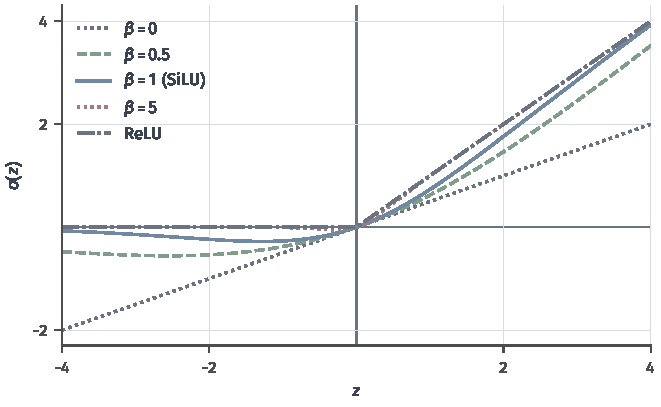
\includegraphics[width=105.412mm]{figures/05-neural-network-models/00-shared/matplotlib/ffn-activation-swish/figure.pdf}
  \caption{Swish在不同$\beta$下的函数图像。$\beta=0$给出线性函数$z/2$，$\beta=1$就是SiLU，较大的$\beta$逐渐形成接近ReLU的响应。图中参数固定为$0,0.5,1,5$，ReLU用作极限参照；它不展示可学习$\beta$在某次训练中的实际轨迹。}
  \label{fig:ffn-activation-swish}
\end{figure}

\term{高斯误差线性单元}（Gaussian error linear unit, GELU）采用标准正态累积分布函数$\Phi$作为保留系数：
\begin{equation}
  \operatorname{GELU}(z)=z\Phi(z),
  \qquad \operatorname{GELU}'(z)=\Phi(z)+z\varphi(z)\text{。}
  \label{eq:ffn-smooth-gates}
\end{equation}
其中$\varphi(z)=\exp(-z^2/2)/\sqrt{2\pi}$是标准正态密度。GELU在全实数上平滑，但公式中的分布函数为每个输入确定一个保留系数，执行时采用确定响应。它常作为Transformer前馈模块的激活选择，平滑性保证局部导数连续，训练所得解的损失仍由完整目标与更新过程决定。常见近似为$z s(1.702z)$，或者
\begin{equation}
  \operatorname{GELU}(z)\approx
  \frac z2\left(1+\tanh\!\left[\sqrt{\frac2\pi}
  (z+0.044715z^3)\right]\right)\text{。}
  \label{eq:ffn-gelu-approximation}
\end{equation}
使用哪种近似会改变实际数值与导数，这会影响复现结果，因此模型记录需要标明精确式或近似式；GELU与SiLU的保留系数不同\scite{hendrycks2016gelu}

保留系数的含义可以用几个输入看清。标准正态分布关于零对称，所以$\Phi(0)=1/2$；此时输入恰为零，GELU输出仍为零。取$z=1$和$z=-1$时，保留系数分别约为$0.8413$和$0.1587$，输出因而约为$0.8413$和$-0.1587$。较大的正输入对应接近一的系数，较大的负输入对应接近零的系数；负输入没有像ReLU那样一律被置零，而是随输入位置受到不同程度的缩放。

\term{Mish函数}进一步用Softplus和Tanh形成平滑的保留系数\scite{misra2019mish}其定义为
\begin{equation}
  \operatorname{Mish}(z)=z\tanh(\operatorname{Softplus}(z))\text{。}
  \label{eq:ffn-mish}
\end{equation}
令$t=\tanh(\operatorname{Softplus}(z))$，乘积与链式法则给出导数$t+zs(z)(1-t^2)$。Mish在负半轴保留一段负响应，负尾部趋近零，正端接近线性，可作为视觉网络或普通隐藏层的另一种平滑选择；原论文的比较是在指定模型与数据上进行的，这些设置决定了所报告收益的适用范围。

这些平滑函数需要指数、Tanh或正态分布函数计算。若希望用简单分段运算近似SiLU，可使用\term{硬Swish}（hard swish, Hardswish）。MobileNetV3在面向移动端的结构中使用这种响应\scite{howard2019mobilenetv3}其定义为
\begin{equation}
  \operatorname{Hardswish}(z)=z\frac{\operatorname{ReLU6}(z+3)}6
  =\begin{cases}
    0,&z\leq-3,\\
    z(z+3)/6,&-3<z<3,\\
    z,&z\geq3\text{。}
  \end{cases}
  \label{eq:ffn-hardswish}
\end{equation}
它在中间区间的导数为$(2z+3)/6$，在两端分别为$0$和$1$，在$\pm3$处不具有唯一导数。这里的门采用斜率$1/6$的硬Sigmoid形式，与前面斜率$1/4$的版本具有不同的线性段与截断点。实际速度取决于算子与硬件实现，而不只取决于公式中出现几个基本运算。

\begin{figure*}[htb]
  \centering
  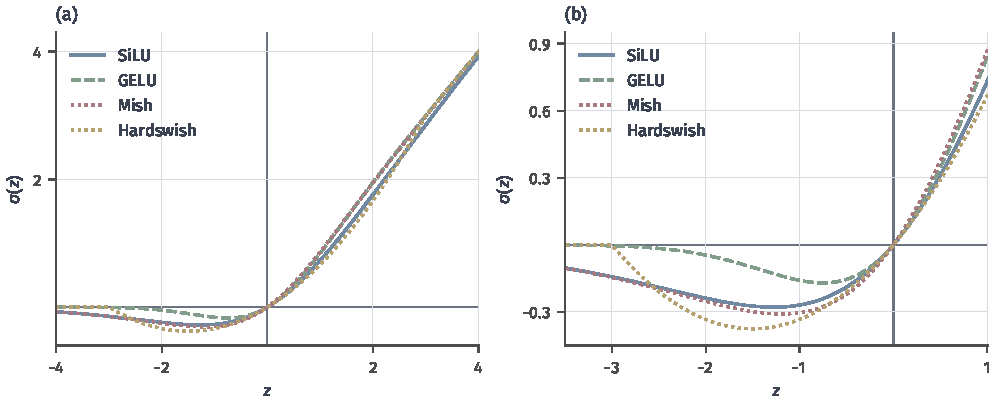
\includegraphics[width=159.059mm]{figures/05-neural-network-models/00-shared/matplotlib/ffn-activation-smooth/figure.pdf}
  \caption{SiLU、GELU、Mish与Hardswish。左图展示整体响应，右图放大原点附近的负值和过渡区域；GELU按标准正态累积分布函数计算响应。它们在正端接近线性，但负区间的形状和拐点不同。SiLU、GELU与Mish平滑，Hardswish含有分段边界；两图使用不同坐标范围以显示细节。}
  \label{fig:ffn-activation-smooth}
\end{figure*}

\subsubsection{Maxout与Softmax}
\label{sec:ffn-activation-vector}

以上函数分别作用于一个标量。若希望一个单元从若干候选响应中选择最大者，可以使用\term{Maxout单元}（maxout unit）：它先计算$K$个仿射响应，再取最大值，响应的分段形状由权重学习得到。对于输入$\bm{u}\in\mathbb{R}^{m}$，其定义为
\begin{equation}
  z_k=\bm{w}_k^{\top}\bm{u}+b_k,
  \qquad h=\max_{1\leq k\leq K}z_k\text{，}
  \label{eq:ffn-maxout}
\end{equation}
其中每个$\bm{w}_k\in\mathbb{R}^{m}$、$b_k\in\mathbb{R}$都参与学习。只有一个严格最大响应时，梯度传给这一响应；多个响应并列最大时需约定分配方式。固定一个响应为零、另一个为$\bm{w}^{\top}\bm{u}+b$，就得到ReLU这一特殊形式。一个Maxout单元对输入表示为凸分段仿射函数；多层复合还包含可正可负的线性组合，完整网络的凸性须由整体计算判断\scite{goodfellow2013maxout}

Maxout适合希望学习分段响应形状的隐藏单元，也曾与Dropout联合研究。相对于一个普通仿射响应，它有$K$套权重与偏置，参数和响应计算量通常约增至$K$倍，这$K$套响应都要分别计算。梯度的截断由最大值选择决定：长期未被选中的分支可能收不到梯度。它还不再是式\eqref{eq:ffn-hidden-layers}中逐坐标作用于一个仿射响应的激活，反向计算需使用最大值选择对应的规则。

把$K$个得分转换为互斥事件的概率时，可以用\term{归一化指数映射}（softmax）让较大得分对应较大概率，并把概率总和固定为一。
对$\bm{z}\in\mathbb{R}^{K}$，其第$k$个输出为
\begin{equation}
  p_k=\operatorname{softmax}(\bm{z})_k
  =\frac{\exp(z_k)}{\sum_{j=1}^{K}\exp(z_j)},
  \qquad \sum_{k=1}^{K}p_k=1\text{。}
  \label{eq:ffn-softmax-activation}
\end{equation}
每个概率依赖全部输入坐标；画一维响应曲线时，需要固定其余坐标。
Jacobian矩阵描述每项概率对各得分的变化：
$\partial p_k/\partial z_j=p_k(\mathbb I\{k=j\}-p_j)$。

这里的指示记号$\mathbb I\{k=j\}$在两个索引相等时取$1$，否则取$0$。固定输出索引$k$，当改变的输入也是$z_k$时，分子与分母都会变化；当改变的是另一个$z_j$时，只有共同分母变化。按商的求导规则，两种情况分别为
\[
  \begin{aligned}
    \frac{\partial p_k}{\partial z_k}
      &=\frac{\exp(z_k)\sum_{i=1}^{K}\exp(z_i)-\exp(2z_k)}
              {\left(\sum_{i=1}^{K}\exp(z_i)\right)^2}
        =p_k(1-p_k),\\
    \frac{\partial p_k}{\partial z_j}
      &=-\frac{\exp(z_k)\exp(z_j)}
              {\left(\sum_{i=1}^{K}\exp(z_i)\right)^2}
        =-p_kp_j,\qquad j\ne k\text{。}
  \end{aligned}
\]
两种结果合在一起，就是上面的指示记号形式；Jacobian矩阵的第$k$行、第$j$列记录的正是这一变化率。
提高本类得分会增大本类概率，提高另一类得分则经共同分母降低本类概率；
若固定一个输入得分$z_j$，再把所有输出坐标$k=1,\ldots,K$对它的导数相加，则
\[
  \sum_{k=1}^{K}\frac{\partial p_k}{\partial z_j}
  =\sum_{k=1}^{K}p_k\mathbb I\{k=j\}
      -p_j\sum_{k=1}^{K}p_k
  =p_j-p_j=0\text{。}
\]
第一项只留下$k=j$的那一项，第二项利用概率总和为$1$。
各输出导数之和为零，与概率总和保持为一相符
（可参考\BookChapterRef{chap:mathematical-analysis}{卷1《数学准备：计算、分析与几何》的“测度与分析”章}）。
Softmax适合互斥多分类输出和需要归一化权重的模块；多标签输出则通常分别使用Sigmoid。
训练时把Softmax与交叉熵合并，可以得到更直接且数值稳定的梯度，下一小节将展开。

\begin{figure*}[htb]
  \centering
  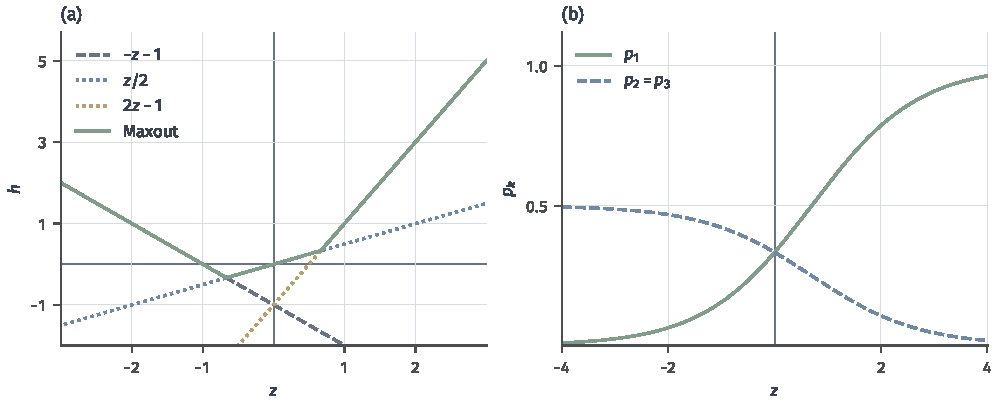
\includegraphics[width=159.059mm]{figures/05-neural-network-models/00-shared/matplotlib/ffn-activation-vector/figure.pdf}
  \caption{Maxout和Softmax的一维观察方式。左图取三个仿射候选$-z-1$、$0.5z$和$2z-1$，粗实线是它们的最大值包络；它展示固定参数后沿一维输入的Maxout响应。右图固定三类得分为$(z,0,0)$，绘出三项Softmax概率，其中$p_2=p_3$，用同一条曲线标注。这些切片不能代表所有输入与参数下的唯一函数图像。}
  \label{fig:ffn-activation-vector}
\end{figure*}

\subsubsection{激活函数的比较与选择}
\label{sec:ffn-activation-selection}

表~\ref{tab:ffn-activation-bounded}归纳了前面的有界响应与整流函数，表~\ref{tab:ffn-activation-smooth}补充指数型、自门控与向量变换。两表中的输出范围对应该层的任务约束，导数特点说明哪些输入区间能传递学习信号，参数与随机机制则说明响应怎样取得。曲线比较只呈现固定参数下的形状，训练还包括参数更新或随机采样。



\begin{table*}[htb]
  \centering
  \small
  \begin{tabularx}{\linewidth}{@{}l l X X@{}}
    \toprule
    函数 & 输出范围 & 导数与参数特点 & 适用场景及主要边界 \\
    \midrule
    ELU & $(-\alpha,+\infty)$ & 负端导数趋零，$\alpha$固定 & 允许负响应；零均值没有无条件保证 \\
    SELU & $(-\kappa\alpha,+\infty)$ & 固定缩放与负指数响应 & 自归一化MLP；需配套统计条件 \\
    Softplus & $(0,+\infty)$ & 平滑，导数为Sigmoid & 正尺度输出、平滑隐藏层；无精确零 \\
    Swish／SiLU & 依赖$\beta$ & $\beta$固定或学习，SiLU取$1$ & 平滑隐藏层、前馈模块；局部可非单调 \\
    GELU & 有负下界，正端无界 & 平滑，精确式或近似式 & Transformer前馈模块；非随机采样 \\
    Mish & 有负下界，正端无界 & 平滑，复合运算 & 视觉或其他隐藏层；收益需验证 \\
    Hardswish & $[-3/8,+\infty)$ & 两个分段边界 & 移动端响应；速度取决于实现 \\
    Maxout & 依赖候选仿射响应 & 选中分支获梯度，$K$套参数 & 学习分段函数；分支可能少获梯度 \\
    Softmax & 概率单纯形内部 & 联合依赖全部得分 & 互斥类别、归一化权重；非逐坐标激活 \\
    \bottomrule
  \end{tabularx}
  \caption{指数型、自门控与向量变换的比较。Swish在$\beta=0$时是线性函数；其余正$\beta$情形具有有限负下界。Softmax按$K\geq2$书写，输出各项严格为正且总和为$1$。表中的平滑性描述固定参数的标量函数，不能替代整条计算路径的可微性检查。}
  \label{tab:ffn-activation-smooth}
\end{table*}

若该层预测概率或正尺度，输出约束通常决定选择：互斥类别用Softmax，多个可共存标签分别用Sigmoid，正尺度可以用Softplus。若该层构造隐藏表示，则需要比较非线性、活动范围与梯度。ReLU提供简单的分段响应，Leaky ReLU与PReLU保留负梯度，GELU与SiLU提供平滑过渡；SELU与特定初始化和统计条件配套，采用它时需要同时确定这些条件。

计算成本也必须放回实现环境。分段线性函数少用指数等运算，但向量化、融合算子和内存访问可能改变实际耗时。平滑函数可用于需要连续导数的模型，其导数仍可能在某些输入区间很小；增加可学习斜率也可能改变初始化时的合适尺度。比较预测性能时，应固定数据划分、结构和评价口径，并说明是否重新调节学习率与初始化，才能区分激活变化和配套设置变化的影响。

% 历史开篇的两条完整边注文献需要与段落一起容纳。
\Needspace{16\baselineskip}
\subsubsection{从阈值单元到平滑门控：发展脉络}
\label{sec:ffn-activation-history}

McCulloch与Pitts在1943年把神经活动的“全或无”性质写成阈值单元；Rosenblatt在1958年的感知机工作中进一步讨论了连接如何从样本中调整\scite{mcculloch1943,rosenblatt1958}这些早期模型用单元的开关组合表达判定。硬阈值便于表达逻辑关系，但其普通导数几乎处处为零，无法直接承担本章所用的多层梯度学习。

当隐藏层需要通过损失学习表示时，连续响应提供了可用的局部导数。Rumelhart、Hinton与Williams在1986年的反向传播论文中使用Logistic响应，展示了隐藏单元怎样随训练形成特征。这一工作将可微的连续响应与隐藏表示的学习结合起来，使激活函数的选择与训练机制紧密相连\scite{rumelhart1986}

Sigmoid与Tanh随后也暴露出深层训练的尺度问题：两端饱和时，导数会变小，Sigmoid在原点附近的输出又以二分之一为中心。2010年Glorot与Bengio的工作把激活响应与初始化放在一起分析，考察了单元可导之外的传播条件：活动值和梯度经过多层之后是否仍有合适尺度。Tanh把输出中心移到零附近，但仍保留两端饱和的边界\scite{glorot2010initialization}

这里的“中心”指响应曲线在原点附近的位置：Sigmoid满足$s(0)=1/2$，Tanh满足$\tanh(0)=0$，后者的正负输出范围还关于零对称。若输入分布本身偏向一侧，输出仍可能有非零均值；只有加入前面所述的对称输入分布等条件，曲线的对称性才能进一步推出输出均值为零。

这项工作的对照还表明，即使保留同一种激活，改变权重初始化方式也会改变各层活动值与梯度的尺度。选择激活函数时，因而还要把初始化和层深放在一起考察：一条曲线的局部斜率不足以描述整条网络的训练状态。第~\ref{sec:ffn-initialization}节将从信号的二阶矩出发解释这种配合，区分Tanh的中心响应与ReLU的半轴截断。

整流函数让设计重点转向稀疏响应和正半轴上的线性传播。Nair与Hinton在2010年研究了受限玻尔兹曼机中的整流单元；Glorot、Bordes与Bengio在2011年进一步比较深层前馈网络的整流与Tanh响应。这两项工作分别在生成模型与深层判别网络中展示了整流响应的作用。正半轴不饱和缓解了一类梯度衰减，负半轴的零导数又促使后续方法保留泄漏斜率或允许负响应\scite{nair2010rectifiers,glorot2011rectifiers}

较新的分支把注意力转向平滑过渡与输入相关的门控。2016年的GELU按输入幅度平滑加权；2017年的Swish工作通过函数搜索研究自门控响应，并与ReLU比较。两者都保留较大的正响应，同时用平滑过渡替代正负区域之间的硬切换\scite{hendrycks2016gelu,ramachandran2017swish}

本节介绍的带斜率变体、指数响应和硬近似，分别延伸了可学习形状、信号尺度与计算成本这些方向。历史上的改进解决的是特定结构和训练设置中的问题；这些设置也构成今天复用相应结果时的条件。Sigmoid和Softmax在概率输出中的用途，则由预测对象决定，并不因隐藏层采用ReLU或平滑门控而消失。

\subsection{输出和学习目标}
\label{sec:ffn-output-objectives}

前面的隐藏层把输入变成了表示$\bm h^{(L)}$。但表示本身不是答案：要让网络完成任务，还必须回答两个问题——网络末端输出的数字\emph{代表什么}，以及用什么标准\emph{评判}这些数字与真实标签的差距。这部分末端计算称为输出头（output head）：它先用可学习的权重和偏置从隐藏表示算出若干个原始得分$\bm a$，再用一个由任务性质决定的变换$g$把得分变成有意义的预测量。

之所以需要不同的输出头，是因为不同任务要预测的对象在数学性质上不同：房价可以是任意实数，邮件是否垃圾邮件是一个“是/否”概率，手写数字是十个互斥类别中的一个，一篇文章的主题标签则可以同时成立多个。用同一套末端处理这些不同对象，要么得到没有意义的数值（比如对类别号直接做平方误差），要么无法表达必要的约束（比如概率必须落在$[0,1]$且互斥类别概率之和为$1$）。因此输出变换$g$不是可以随意选择的装饰，而是任务语义的一部分；与之配套的损失函数则决定训练信号。训练时可以让隐藏层与输出头一起调整，也可以在复用已训练网络时冻结隐藏层、只学习新任务的输出头。

同一组隐藏坐标可以接不同的输出头。图~\ref{fig:ffn-output-heads}比较连续数值、二分类、多类、多标签和表示输出五种方案；各头有各自的参数与损失，图中分支表示可替换的选择。下面按“原始得分长什么样、变换成什么预测量、用什么损失计分、如何据此作决策”这条统一线索，依次介绍这些输出头。

\begin{figure*}[!htb]
  \centering
  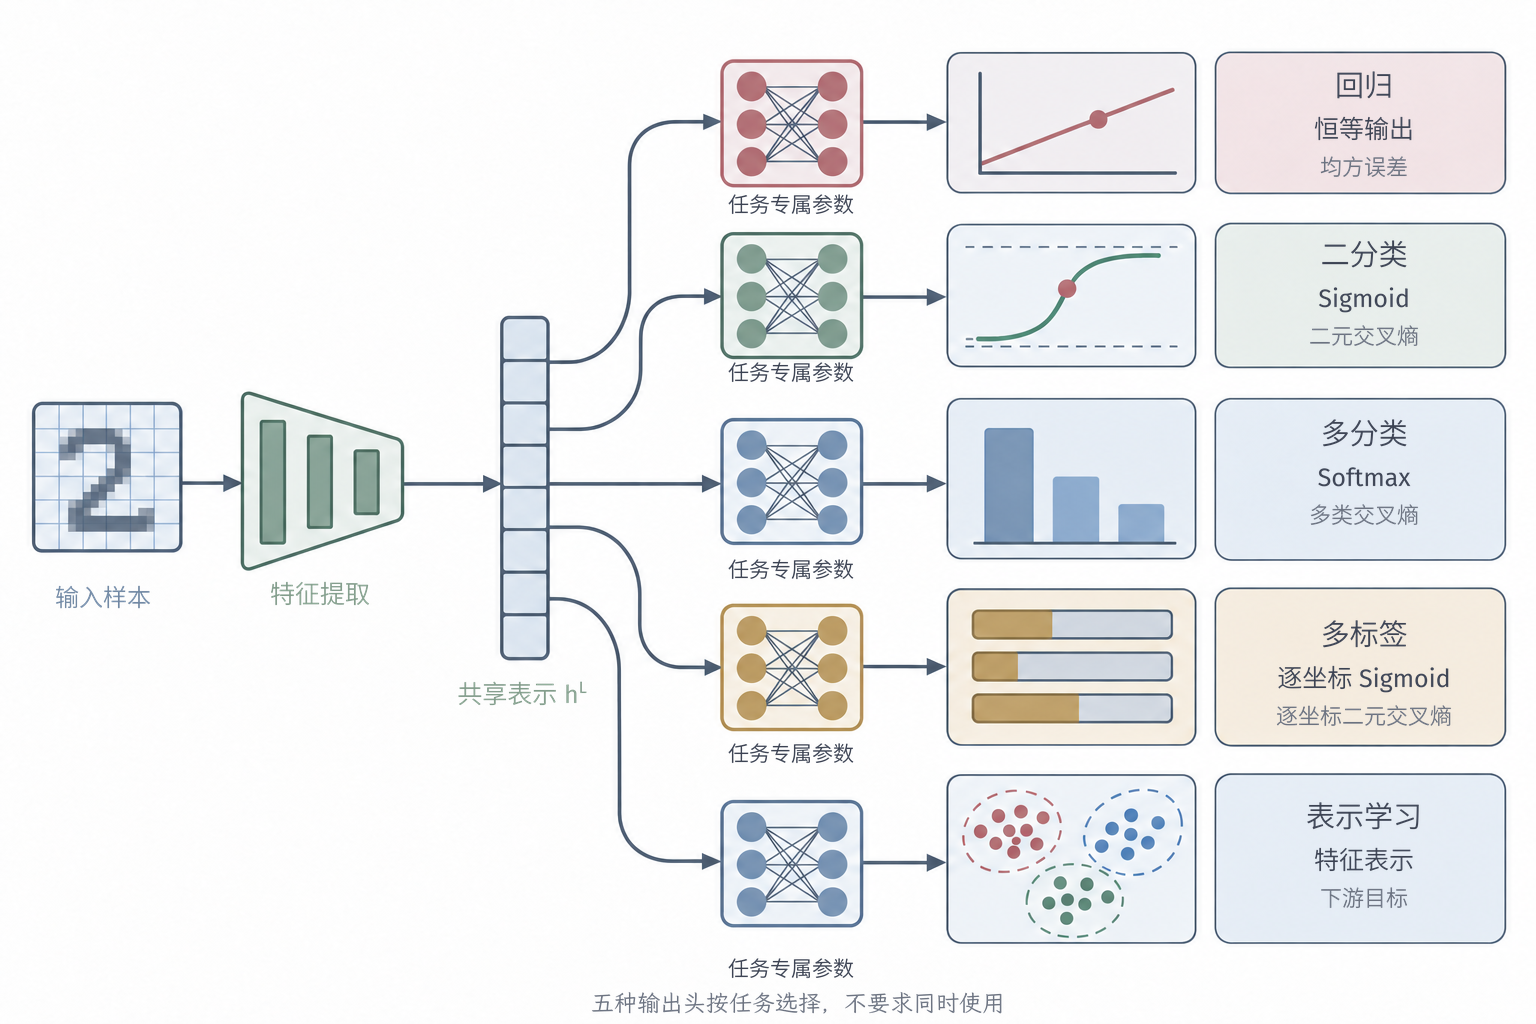
\includegraphics[width=130.048mm]{figures/05-neural-network-models/00-shared/generated/ffn-output-heads/figure.png}
  \caption{共同的前馈结构与五种可替换的输出头。左侧输入单元经隐藏单元形成$\bm{h}^{(L)}$；汇合线传递整组隐藏坐标，不执行求和。右侧单元产生各任务自己的原始得分，每个单元都读取全部隐藏坐标，并具有独立的输出权重与偏置。回归与二分类头只需一个得分；多类分类头联合归一化，多标签分类头逐坐标变换；表示头产生由下游任务约束的表示。向量头仅画三个坐标示意，实际维度由任务决定。右侧文字区分预测量与训练目标，隐藏激活无需与输出变换相同。}
  \label{fig:ffn-output-heads}
\end{figure*}

\subsubsection{回归：预测连续数值}
\label{sec:ffn-output-regression}

回归预测连续数值，例如经过单位缩放的房价。对标量目标$y\in\mathbb R$，输出头只需产生一个得分$a$，即$q=1$。采用恒等变换$g(a)=a$时，预测值为$\widehat y=a$，可用平方损失衡量它与目标的偏差：
\begin{equation}
  \ell(a,y)=\frac12(a-y)^2,
  \qquad \frac{\partial\ell}{\partial a}=a-y\text{。}
  \label{eq:ffn-regression-loss}
\end{equation}
系数$1/2$简化导数，不改变仅有该损失时的最优预测。若目标为$2.5$、当前预测为$2$，损失为$0.125$，输出导数为$-0.5$；沿负梯度方向调整输出会使它增大并接近目标。多个连续目标可用向量输出和$\frac12\lVert\bm a-\bm y\rVert_2^2$，各坐标的单位与尺度应在数据处理或损失权重中考虑。若要求严格正值预测，可以先令$\widehat y=\operatorname{Softplus}(a)$，再对变换后的预测计算损失。

\subsubsection{二分类：预测一个正类概率}
\label{sec:ffn-output-binary}

二分类判断一个事件是否成立，例如邮件是否属于垃圾邮件。令$y\in\{0,1\}$，其中$1$表示正类。这里希望网络给出的不是一个无界实数，而是“属于正类的概率”，概率必须落在$[0,1]$区间。但输出层算出的原始得分$a$可以是任意实数（很大的正数或很负的数），因此需要一个把整条实数轴单调压进$(0,1)$的变换。输出头产生一个实数$a$，经Sigmoid得到
\[
  p=s(a),\qquad P_{\bm\theta}(y=1\mid\bm x)=p,\qquad
  P_{\bm\theta}(y=0\mid\bm x)=1-p\text{。}
\]
$a$称为\term{logit}，即对数几率$\log(p/(1-p))$；它可以取任意实数，$p$才是正类概率。在这个伯努利模型下，正确标签的概率为$p^y(1-p)^{1-y}$，取负对数得到二元交叉熵：
\begin{equation}
  \begin{aligned}
    \ell(a,y)
      &=-y\log p-(1-y)\log(1-p)\\
      &=\log(1+\exp(a))-ya\text{。}
  \end{aligned}
  \label{eq:ffn-binary-cross-entropy}
\end{equation}
第二行利用$\log p=a-\log(1+\exp(a))$与$\log(1-p)=-\log(1+\exp(a))$，把两个对数项合并。对这一原始得分形式求导，就得到后续反向传播所用的起点：
\[
  \frac{\partial\ell}{\partial a}
  =\frac{\exp(a)}{1+\exp(a)}-y=p-y\text{。}
\]
例如正例的$p$从$0.8$降到$0.2$时，损失从约$0.2231$增到$1.6094$，说明损失会区分分给正确标签的概率。预测类别还需规定阈值$\tau$，如按$p\geq\tau$判正类；阈值应结合误判代价与验证指标选择。学习时使用连续损失，作出类别决策时才应用阈值。

\subsubsection{互斥多分类：预测一个类别}
\label{sec:ffn-output-multiclass}

若样本恰好属于$K$类中的一类，例如一张数字图像对应“0到9”中的某一个数字类别，就让输出头产生$K$个得分$a_1,\ldots,a_K$，即$q=K$。互斥意味着这$K$个概率必须满足两个条件：每个都非负，且加起来恰好等于$1$（样本必定属于其中某一类）。如果对每个得分分别用Sigmoid，得到的$K$个数之间没有这种竞争关系，它们之和既不等于$1$、也无法直接解释成一个概率分布。Softmax通过一次共同归一化来建立这种竞争：标签为$y\in\{1,\ldots,K\}$，Softmax把得分共同转换为互斥类别的概率，并按最大概率判类：
\begin{equation}
  p_k=\frac{\exp(a_k)}{\sum_{j=1}^{K}\exp(a_j)},
  \qquad \sum_{k=1}^{K}p_k=1,\qquad
  \widehat y=\operatorname*{arg\,max}_{k}p_k\text{。}
  \label{eq:ffn-multiclass-output}
\end{equation}
最大概率并列时需预先固定决策规则。正确标签的概率是$p_y$，取负对数得到多类交叉熵：
\begin{equation}
  \ell(\bm{a},y)=-\log p_y
  =-a_y+\log\sum_{j=1}^{K}\exp(a_j)\text{。}
  \label{eq:ffn-multiclass-cross-entropy}
\end{equation}
对$a_k$求导时，$-a_y$贡献$-\mathbb I\{y=k\}$，其中指示函数在$y=k$时为$1$，否则为$0$；对数求和项贡献$\exp(a_k)/\sum_j\exp(a_j)=p_k$。两项相加，得分梯度就是$p_k-\mathbb I\{y=k\}$。因此正确类得分的负梯度方向为正，其他类为负；这些信号怎样调整输出权重及隐藏表示，将由反向传播计算。

\subsubsection{多标签分类：预测多个二值结果}
\label{sec:ffn-output-multilabel}

同一文档可以同时属于“技术”和“教育”，这类任务需要分别判断多个标签是否成立。与互斥多分类相反，这里的标签之间没有竞争关系：一个标签成立不会挤占其他标签成立的可能，因此不能用Softmax强制概率之和为$1$，而应对每个标签各设一个独立的“是/否”判断。\term{多标签分类}（multi-label classification）使用目标$\bm y\in\{0,1\}^{K}$，输出头对每个得分分别使用Sigmoid，再把各标签的二元交叉熵相加：
\begin{equation}
  \begin{aligned}
    p_k&=s(a_k),\\
    \ell(\bm{a},\bm{y})
      &=\sum_{k=1}^{K}\bigl[-y_k\log p_k-(1-y_k)\log(1-p_k)\bigr]\\
      &=\sum_{k=1}^{K}\bigl[\log(1+\exp(a_k))-y_k a_k\bigr]\text{。}
  \end{aligned}
  \label{eq:ffn-multilabel-loss}
\end{equation}
这些概率不必加起来等于$1$。例如$\bm p=(0.8,0.7,0.1)^{\top}$，按各标签的阈值$0.5$决策，会选出前两个标签。每一项沿用二分类损失，所以每个得分的梯度仍为$p_k-y_k$；不同标签也可以分别选择阈值。这两种任务都可输出$K$维向量，标签是否允许共存决定使用Softmax还是逐坐标Sigmoid。

\subsubsection{表示输出：由下游目标提供约束}
\label{sec:ffn-output-representation}

输出也可以继续交给其他模块使用。例如，下游模块需要的表示维度与$\bm h^{(L)}$不同，输出头便先把它映射为$\bm a\in\mathbb R^q$，再作为表示$\bm r$供分类、比较或重建使用。可以直接取$\bm r=\bm a$；若任务只比较向量方向，则在$\bm a\neq\bm0$时归一化为
\begin{equation}
  \bm{r}=\frac{\bm{a}}{\lVert\bm{a}\rVert_2}\text{。}
  \label{eq:ffn-normalized-representation}
\end{equation}
例如$(3,4)^{\top}$变为$(0.6,0.8)^{\top}$，保留方向、去掉整体长度差异。归一化只规定长度，表示应保留什么信息仍需由使用目标确定：接分类头时由分类损失约束表示，用于重建时由重建误差约束表示。联合训练时，这些损失的梯度经过下游模块传回表示网络，使输出坐标接受使用任务的约束。

\subsubsection{从单样本损失到训练目标}
\label{sec:ffn-empirical-objective}

前面已经规定了一条样本怎样预测、怎样计分，学习则要让同一组参数服务于整个训练集。设$S=((\bm x_i,\bm y_i))_{i=1}^{n}$，标量标签按对应任务书写，网络对第$i$个输入产生原始得分$\bm a_i(\bm\theta)$。汇总各样本损失，并加入可选的参数惩罚，得到
\begin{equation}
  J_S(\bm{\theta})=
  \frac1n\sum_{i=1}^{n}\ell\!\left(\bm{a}_i(\bm{\theta}),\bm{y}_i\right)
  +\lambda\Omega(\bm{\theta})\text{。}
  \label{eq:ffn-training-objective}
\end{equation}
这里$\ell$已包含任务的输出变换，$\Omega$是参数惩罚，$\lambda\geq0$控制惩罚强度；表示输出的损失则来自相连的下游目标。固定隐藏层时，其参数保持不变，只调整输出头；联合训练时，两部分参数共同参与同一目标的更新。输出范围由$g$规定，训练依据由损失给出；对于分类任务，阈值或最大概率规则再把预测用于具体决策。

\section{参数学习}
\label{sec:ffn-learning}

结构和损失规定了“网络长什么样、什么算好”，但训练开始时表里还没有填入合适的数值。要真正学到参数，还要解决两个工程与数学上都无法回避的问题。第一个是\emph{起点}：在看到任何数据之前，权重应当初始化成什么？全部置零看似自然，却会导致致命的对称问题；随机赋值则要进一步考虑数值取多大才合适。第二个是\emph{方向}：网络可能有几百万、上亿个参数，每更新一次，都要知道每个参数应当增大还是减小、变动多少，手工推导显然不可行，这就需要一套能机械执行的求导算法——反向传播。初始化决定从参数空间的哪个位置出发，反向传播决定每一步朝哪个方向走，自动微分则让程序能够自动完成这些求导；至于沿这个方向走多大一步（学习率）、用什么优化策略走，则属于求出梯度之后的优化问题。

\subsection{参数初始化}
\label{sec:ffn-initialization}

初始化要同时满足两个看起来独立、实则相关的要求：让同层单元“各不相同”，并让信号和梯度在层间传播时“尺度不失控”。第一点针对对称性，第二点针对数值幅度。下面先说明为什么这两点都不可省略，再据此结合每层的连接数推导合适的权重方差。

\subsubsection{共同要求：打破对称并控制尺度}
\label{sec:ffn-initialization-common}

先看对称性为什么是致命的。假设一层里所有单元的输入权重、偏置完全相同，并且它们通向下一层的连接也对称，那么无论输入什么，这一层所有单元的输出都相同；反向传播时，它们收到的梯度也完全相同，于是更新之后权重仍然相同。这种对称性一旦建立就会被每一步更新严格保持下去：一个有$64$个单元的隐藏层，实际上永远只在重复计算同一个特征，等价于只有一个单元，网络的容量被白白浪费。全零初始化正是这种完全对称的起点。因此权重必须随机初始化，使各单元一开始就关注不同的输入方向；偏置不参与打破这种方向对称，通常可以置零（或按输出层的需要单独设置）。

打破对称只解决了“各不相同”，还没有解决“取多大”。若权重普遍过大，加权和的绝对值会很大，Sigmoid、Tanh单元随即进入两端几乎水平的饱和区；若权重普遍过小，信号逐层衰减，深层单元的输入几乎相同、难以区分，梯度也会随之变得微弱。合适的幅度应当与该单元读取的输入个数相联系。设输入坐标具有共同且有限的二阶矩$q_{\mathrm{in}}=\mathbb E[u_k^2]$，初始权重独立、均值为零、方差为$v$，整组权重与整组输入独立，偏置为零。把$m$个输入的加权和$z=\sum_{k=1}^{m}w_k u_k$平方展开，有
\[
  \mathbb E[z^2]
  =\sum_{k=1}^{m}\mathbb E[w_k^2u_k^2]
    +2\sum_{k<j}\mathbb E[w_k w_j u_k u_j]\text{。}
\]
对角项为$\mathbb E[w_k^2]\mathbb E[u_k^2]=v q_{\mathrm{in}}$；交叉项含有$\mathbb E[w_k w_j]=0$，即使输入坐标彼此相关也会消失。因此
\begin{equation}
  \mathbb{E}[z^2]=m v q_{\mathrm{in}}\text{。}
  \label{eq:ffn-initial-signal-scale}
\end{equation}
若激活近似保留预激活的二阶矩，取$m v\approx1$就使本层输出与输入的二阶矩接近；激活进一步压缩或截断响应时，还要计入相应因子。

输入连接数$m=d_{\ell-1}$称为\term{fan-in}；同一输入坐标通向的输出连接数$d_\ell$称为\term{fan-out}。前者决定一个输出汇总多少输入，后者决定一个输入在反向计算中接收多少下游贡献。

\subsubsection{饱和激活的尺度：Glorot初始化}
\label{sec:ffn-initialization-saturating}

对于前面讨论的饱和激活，过大的初始预激活容易进入小导数区域。增大权重虽然能放大仿射结果，也可能把更多单元推入饱和区，因此不能只靠放大权重补偿小导数。先以Tanh原点附近的近似单位斜率为基准，估计前、后两个方向的传播尺度。

记最终标量损失对本层输出预激活$z_j$的敏感度为$\gamma_j$，其共同二阶矩为$q_{\mathrm{back}}$。一个输入$u_k$接收$d_\ell$个输出的影响，链式法则给出
\[
  \widetilde\gamma_k
  :=\frac{\partial\ell}{\partial u_k}
  =\sum_{j=1}^{d_\ell}(\bm W_\ell)_{j,k}\gamma_j\text{。}
\]
暂把本层权重与整组下游敏感度视为独立，平方展开中的交叉项便消失，每个对角项为$v q_{\mathrm{back}}$，得到$\mathbb E[\widetilde\gamma_k^2]\approx d_\ell v q_{\mathrm{back}}$。这里的独立性是忽略实际依赖的尺度近似，故对真实网络使用近似等号。

前向和后向的传播因子分别为$d_{\ell-1}v$与$d_\ell v$。两侧宽度不同时，不能用同一个$v$让它们都等于$1$；一种折中是令两因子的算术平均为$1$，即$((d_{\ell-1}+d_\ell)/2)v=1$。\term{Glorot初始化}（Glorot initialization，也称Xavier初始化）由此采用
\begin{equation}
  \begin{aligned}
    v&=\frac{2}{d_{\ell-1}+d_\ell},\\
    (\bm{W}_\ell)_{j,k}&\sim
    \mathcal{U}\!\left[-\sqrt{\frac{6}{d_{\ell-1}+d_\ell}},
    \sqrt{\frac{6}{d_{\ell-1}+d_\ell}}\right]\text{。}
  \end{aligned}
  \label{eq:ffn-glorot-initialization}
\end{equation}
其中$\mathcal U$表示均匀分布。对$a>0$，$\mathcal U[-a,a]$的方差为$\frac1{2a}\int_{-a}^{a}t^2\,\mathrm dt=a^2/3$，令它等于上述$v$，就得到式中的端点；也可以采用同方差的零均值正态分布。

改变激活时，还可按其传播作用调整初始权重的标准差，这个调整系数称为激活增益；标准差乘一个系数时，方差要乘其平方。Sigmoid的中心斜率更小，且具有非零输出中心，因此上述单位斜率近似不能直接覆盖它的传播；Glorot与Bengio的分析也考察了这些因素及饱和问题\scite{glorot2010initialization}

\subsubsection{ReLU及其变体：补偿被截断的响应}
\label{sec:ffn-initialization-rectifiers}

对于ReLU，需要补偿负半轴被截断的平方幅度。若预激活$z$关于零对称，正、负半轴的平方贡献相等；零点的平方贡献为零，所以即使零点具有正概率质量，仍有
\[
  \mathbb{E}[\rho(z)^2]=\frac12\mathbb{E}[z^2]\text{。}
\]
这是二阶矩关系；ReLU输出通常有正均值，方差还要减去均值平方。结合式\eqref{eq:ffn-initial-signal-scale}，激活后的二阶矩为$q_{\mathrm{out}}=(m v/2)q_{\mathrm{in}}$；要使$q_{\mathrm{out}}\approx q_{\mathrm{in}}$，可取$v\approx2/m$。相应的\term{He初始化}（He initialization，也称Kaiming初始化）采用
\begin{equation}
  (\bm{W}_\ell)_{j,k}\sim
  \mathcal{N}\!\left(0,\frac{2}{d_{\ell-1}}\right)\text{。}
  \label{eq:ffn-he-initialization}
\end{equation}

在同一对称分布下，初始化时若负半轴斜率固定为$\alpha$，正、负半轴分别贡献原二阶矩的$1/2$和$\alpha^2/2$，总因子为$(1+\alpha^2)/2$。因此，Leaky ReLU或PReLU初始斜率对应的前向权重方差为$2/((1+\alpha^2)d_{\ell-1})$；PReLU开始学习斜率后，这一初始补偿尺度也可能改变。

后向还需考察局部回传系数的平方平均。若预激活关于零对称且零点概率为零，ReLU两侧的系数平方分别为$1$和$0$，平均为$1/2$；带泄漏时为$(1+\alpha^2)/2$。在局部回传系数、权重与下游敏感度的独立性近似下，将这些因子乘入前面的后向求和估计，就得到把方差分母中的fan-in换成fan-out的方案。若零点有正概率质量，后向因子还取决于零点回传约定，不能仅由对称性确定\scite{he2015rectifiers}

\subsubsection{其他隐藏激活与任务输出：分别设置}
\label{sec:ffn-initialization-other}

其他隐藏激活应按自身响应和实现的增益约定选择尺度，SELU还需沿用前面说明的配套初始化与统计条件。输出层也按自己的运算设置：线性得分层没有半轴截断，无须自动继承ReLU隐藏层的系数$2$；二分类还应关注初始logit是否过大。

使用这些设置时，需要结合输入处理和层宽观察初始活动值与梯度。以上分布与独立性估计描述的是起点，训练后权重、表示和下游敏感度可能相关，仍需根据实际数值判断后续尺度。接下来的反向传播将具体说明这些敏感度怎样计算并用于参数更新。

\subsection{反向传播}
\label{sec:ffn-backpropagation}

初始化解决了起点问题，现在解决训练的核心问题。输出层的参数容易处理：它的输出直接参与损失，预测偏高就把相关权重调低、偏低就调高。隐藏层却不同——我们从不为隐藏单元提供目标值，没有人告诉某个隐藏单元“你此刻应该输出$0.7$”。那么，怎样判断一个深处的隐藏权重应当增大还是减小？

答案来自一个朴素的追问：这个隐藏单元的输出会影响谁？它影响下一层，下一层又影响再下一层……如此一路传到最终损失。因此，最终损失对某个隐藏量的敏感程度，可以沿着这条依赖链\emph{反向}逐层追踪回来：先知道损失对最末端输出有多敏感，再乘以“输出对倒数第二层的局部变化率”，得到损失对倒数第二层的敏感度；如此逐层向内，直到每个参数。这正是微积分中链式法则的系统性应用，称为\term{反向传播}（backpropagation）。

下面把反向传播展开为预激活敏感度、逐层递推、参数梯度与批量汇总四步。采用列向量梯度时，链式法则在矩阵形式上体现为Jacobian转置。

先固定一个样本，把输出变换与损失合为标量函数$\ell(\bm{a},\bm{y})$。用列向量表示梯度，定义
\begin{equation}
  \bm{\delta}^{(L+1)}=\nabla_{\bm{a}}\ell,
  \qquad
  \bm{\delta}^{(\ell)}=\nabla_{\bm{z}^{(\ell)}}\ell
  \quad(\ell=1,\ldots,L)\text{。}
  \label{eq:ffn-delta-definition}
\end{equation}
向量$\bm{\delta}^{(\ell)}\in\mathbb{R}^{d_\ell}$记录损失对本层各预激活坐标的敏感程度。“误差”是这一敏感度的常用名称；其数值来自最终损失的导数，而隐藏层通常没有直接指定的标签。

在可微点，这些敏感度由普通导数给出。ReLU在零点没有普通导数，但训练程序仍需规定遇到该值时怎样回传。本章的ReLU计算采用下面的局部回传系数：
\[
  D_\rho(z)=
  \begin{cases}
    1,&z>0,\\
    0,&z\leq0\text{。}
  \end{cases}
\]
它在两个开半轴上等于ReLU导数，在零点取$0$是一项实现约定，不表示该点存在普通导数。以下递推中，对ReLU原本填写$\rho'(z)$的位置使用$D_\rho(z)$；其他分段激活也要把拐点处的回传规则连同函数定义一起固定。Maxout不是这里的逐坐标激活，它还需规定并列最大时把敏感度分配给哪些分支；这些算子规则是网络计算的一部分。

由式\eqref{eq:ffn-output-map}，输出得分对$\bm{h}^{(L)}$的Jacobian矩阵为$\bm{W}_{L+1}$，
所以损失对最后一个隐藏表示的梯度为$\bm{W}_{L+1}^{\top}\bm{\delta}^{(L+1)}$。
隐藏激活逐坐标作用，其Jacobian矩阵以各坐标导数为对角元素。
把两步链式法则合起来，便得到逐层递推：
\begin{equation}
  \bm{\delta}^{(\ell)}=
  \left(\bm{W}_{\ell+1}^{\top}\bm{\delta}^{(\ell+1)}\right)
  \odot\sigma_\ell'\!\left(\bm{z}^{(\ell)}\right),
  \qquad \ell=L,\ldots,1\text{。}
  \label{eq:ffn-backward-recursion}
\end{equation}
其中$\odot$表示逐坐标乘法。这个递推式虽然紧凑，却只是两步直觉的合并，可以拆开读。第一步$\bm{W}_{\ell+1}^{\top}\bm{\delta}^{(\ell+1)}$回答“后层有多怪罪本层”：后层每个单元的敏感度，按它们与本层各单元的连接权重加权汇总回来，所以用权重矩阵的转置。第二步再逐坐标乘上$\sigma_\ell'(\bm{z}^{(\ell)})$，回答“本层单元自己放行多少”：如果单元正处在激活函数平缓（导数接近零）的区域，即使后层很不满意，这个不满也很难通过该单元传回到它的输入权重。两步合起来，就得到损失对本层预激活值的敏感度。递推中的每个向量维度都是$d_\ell$，因此可逐层核对矩阵形状是否匹配。

这里维度为$d_\ell$的是当前层的递推结果，以及相乘前已经汇总到当前层的向量。后层敏感度$\bm\delta^{(\ell+1)}$本身属于$\mathbb R^{d_{\ell+1}}$；先乘形状为$d_\ell\times d_{\ell+1}$的$\bm W_{\ell+1}^{\top}$，才得到可与本层激活导数逐坐标相乘的$d_\ell$维向量。

参数的导数来自本层仿射运算。对任一层$\ell=1,\ldots,L+1$，第$j$个预激活值对权重$(\bm{W}_\ell)_{j,k}$的导数是$h_k^{(\ell-1)}$，对偏置$(\bm{b}_\ell)_j$的导数是$1$。由此得到
\begin{equation}
  \nabla_{\bm{W}_\ell}\ell
    =\bm{\delta}^{(\ell)}(\bm{h}^{(\ell-1)})^{\top},
  \qquad
  \nabla_{\bm{b}_\ell}\ell=\bm{\delta}^{(\ell)}\text{。}
  \label{eq:ffn-parameter-gradients}
\end{equation}
第一式是一个外积：每条连接的梯度等于目标单元的损失敏感度乘以来源单元的活动值。矩阵形状为$d_\ell\times d_{\ell-1}$，恰好与权重相同。对输入的梯度则为$\nabla_{\bm{x}}\ell=\bm{W}_1^{\top}\bm{\delta}^{(1)}$；即使输入不参与参数更新，这个量也能用于分析预测对输入变化的敏感程度。

输出层的起点由任务决定。采用式\eqref{eq:ffn-regression-loss}时，$\delta^{(L+1)}=a-y$；采用二元交叉熵时，$\delta^{(L+1)}=p-y$；采用多类交叉熵时，第$k$个坐标为$p_k-\mathbb{I}\{y=k\}$，其中$\mathbb{I}$是事件成立时为$1$的指示函数。概率输出与交叉熵合并后得到的简洁导数，是两者配合的结果。若Sigmoid输出后使用平方损失，导数还包含$s'(a)$，此时$p-y$还需乘上述输出变换导数。

图~\ref{fig:ffn-backpropagation}把下面算例的$2$-$3$-$1$网络展开，说明前向值与反向梯度的区别。前向计算提供各层的预激活和表示；反向计算从损失开始，重复利用这些值与局部导数。梯度向上游传播不会改变本次前向预测已经使用的输入，也不会给预测网络增加有向环。

\begin{figure*}[htb]
  \centering
  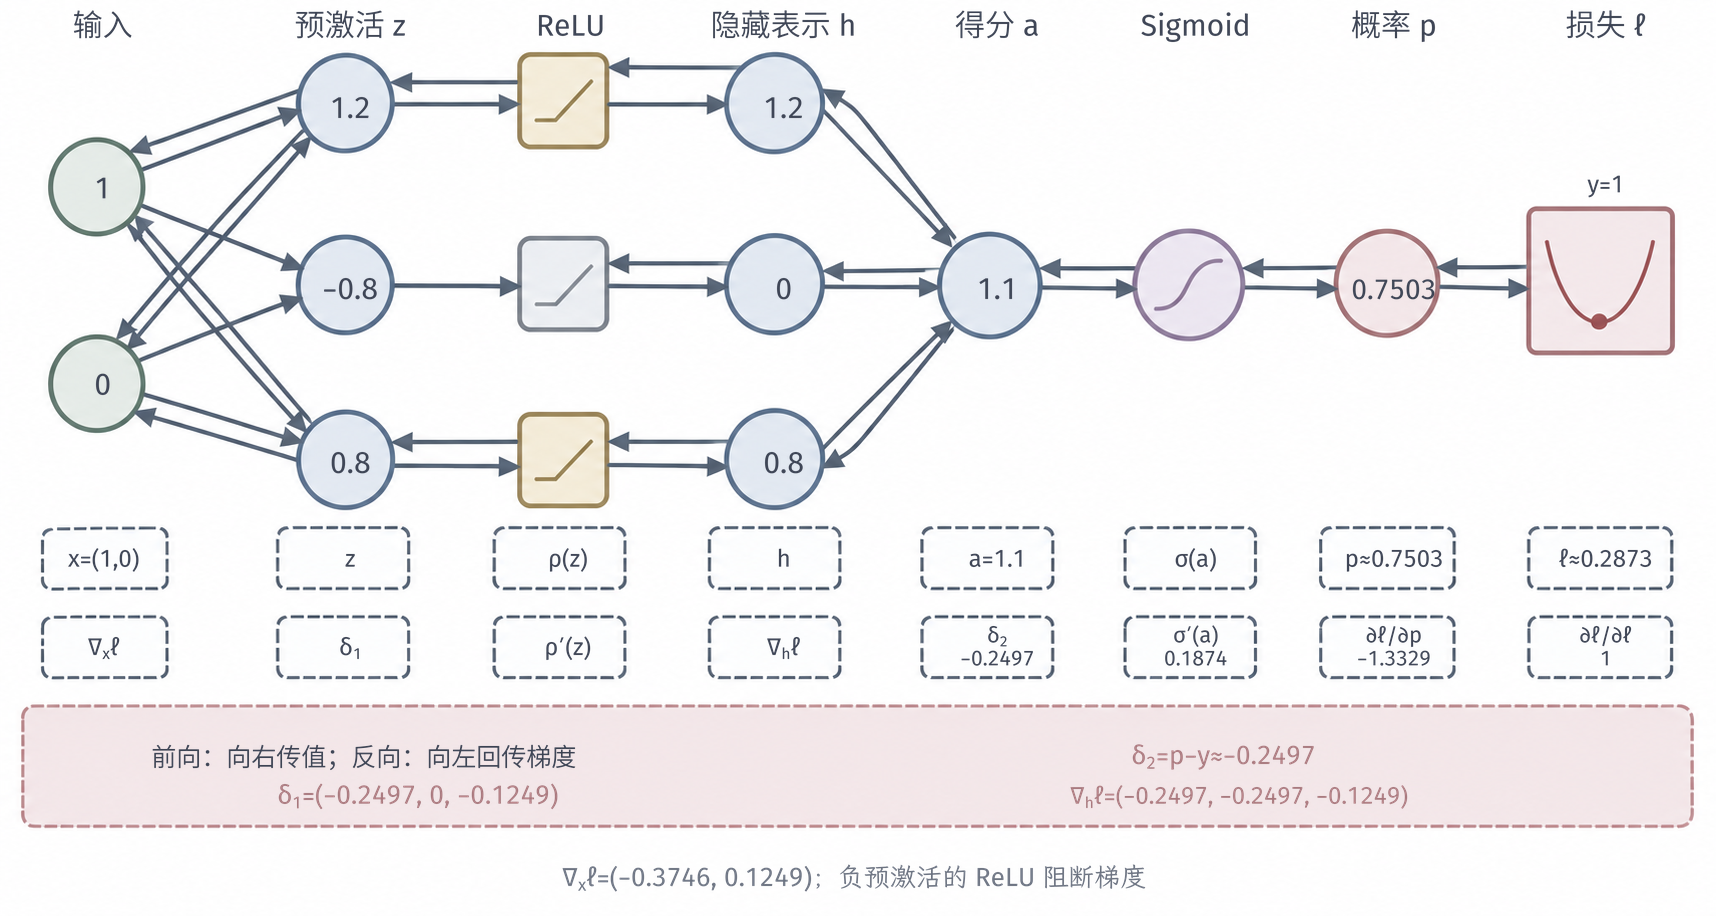
\includegraphics[width=145.288mm]{figures/05-neural-network-models/00-shared/generated/ffn-backpropagation/figure.png}
  \caption{示例~\ref{ex:ffn-numerical-backpropagation}中$2$-$3$-$1$网络的计算图。上方节点和下方第一行给出前向值，第二行及红色汇总给出反向量；箭头方向区分前向传值与反向回传梯度；预激活与隐藏表示是同一隐藏层的两种数值，不是两个隐藏层。下方红色虚线按向量形式汇总梯度，坐标顺序与上方节点从上到下一致。第三个单元通过输出权重$0.5$收到梯度，第二个单元的梯度被负半轴上的ReLU截断。数值按更新前参数计算，梯度和概率保留四位小数。}
  \label{fig:ffn-backpropagation}
\end{figure*}

\begin{example}[一次前向与反向计算]
  \label{ex:ffn-numerical-backpropagation}
  沿用异或的二值输入，使用图~\ref{fig:neural-minimal-mlp}中的$2$-$3$-$1$结构：一个隐藏层含三个ReLU单元，输出得分经Sigmoid变成二分类概率。下面的参数是教学构造，不是已训练好的异或分类器：
  \[
    \begin{aligned}
      \bm{W}_1&=\begin{pmatrix}1&-1\\-1&1\\1&1\end{pmatrix},
      &\bm{b}_1&=\begin{pmatrix}0.2\\0.2\\-0.2\end{pmatrix},\\
      \bm{W}_2&=\begin{pmatrix}1&1&0.5\end{pmatrix},
      &b_2&=-0.5\text{。}
    \end{aligned}
  \]
  对样本$\bm{x}=(1,0)^{\top}$、$y=1$，前向结果为
  \[
    \begin{aligned}
      \bm{z}^{(1)}&=(1.2,-0.8,0.8)^{\top},\\
      \bm{h}^{(1)}&=(1.2,0,0.8)^{\top},\\
      a&=1\times1.2+1\times0+0.5\times0.8-0.5=1.1\text{。}
    \end{aligned}
  \]
  因而$p=s(1.1)\approx0.7503$，二元交叉熵$\ell=-\log p\approx0.2873$。本例三个预激活值都远离ReLU的不可微点，局部导数依次为$1,0,1$。

  输出敏感度为$\delta^{(2)}=p-1\approx-0.2497$。先乘输出权重的转置，再逐坐标乘激活导数，得到
  \[
    \begin{aligned}
      \nabla_{\bm{h}^{(1)}}\ell
        &\approx(-0.2497,-0.2497,-0.1249)^{\top},\\
      \bm{\delta}^{(1)}&\approx(-0.2497,0,-0.1249)^{\top},\\
      \nabla_{\bm{W}_1}\ell&\approx
      \begin{pmatrix}-0.2497&0\\0&0\\-0.1249&0\end{pmatrix},
      &\nabla_{\bm{b}_1}\ell&\approx
      \begin{pmatrix}-0.2497\\0\\-0.1249\end{pmatrix}\text{。}
    \end{aligned}
  \]
  例如第三个隐藏单元的第一条输入权重，其梯度是
  \[
    \frac{\partial\ell}{\partial(\bm{W}_1)_{3,1}}
    =(p-1)\times0.5\times1\times x_1
    \approx-0.1249\text{。}
  \]
  这四个因子依次来自输出损失、输出连接、ReLU局部导数和输入值。输出参数的梯度为$\nabla_{\bm{W}_2}\ell\approx(-0.2997,0,-0.1998)$、$\partial\ell/\partial b_2\approx-0.2497$；继续回传到输入则有$\nabla_{\bm{x}}\ell\approx(-0.3746,0.1249)^{\top}$。第一层第一、第三个单元对$x_2$的权重梯度为零，是因为这个样本的$x_2=0$；第二个单元的输入权重梯度为零，则来自负半轴上的激活导数。两种零梯度有不同原因。

  若仅用该样本、不加正则项，并以学习率$0.1$同时更新所有参数，即每项参数减去$0.1$倍的对应梯度，则更新后的参数为
  \[
    \begin{aligned}
      \bm{W}_1^{(1)}&\approx
        \begin{pmatrix}1.0250&-1\\-1&1\\1.0125&1\end{pmatrix},
      &\bm{b}_1^{(1)}&\approx
        \begin{pmatrix}0.2250\\0.2\\-0.1875\end{pmatrix},\\
      \bm{W}_2^{(1)}&\approx\begin{pmatrix}1.0300&1&0.5200\end{pmatrix},
      &b_2^{(1)}&\approx-0.4750\text{。}
    \end{aligned}
  \]
  参数上标$(1)$表示一次更新。用未舍入的梯度重算该输入，隐藏表示约为$(1.2499,0,0.8250)^{\top}$，得分约为$1.2414$，正类概率约为$0.7758$，损失约为$0.2539$。本次下降只针对更新所用的正例；全部异或样本的总损失与新样本风险，需要分别用相应样本或分布评价。
\end{example}

上面的求导针对一条样本，但一次参数更新是否必须看完整个训练集？如果每次更新都精确计算式\eqref{eq:ffn-training-objective}的数据梯度，就要用当前参数遍历全部$n$个训练样本；在数百万样本的数据集上，这意味着每走一小步都要完整扫描一遍数据，训练慢得无法接受。一个自然的折衷是：每步只随机读取一小部分样本，用这批样本上的平均梯度近似全体样本的梯度。数据较多时，这样既能大幅减少一次更新的计算与中间值存储，又因为频繁更新而往往收敛得更快。为给这种做法规定一种明确含义，并说明“近似”在什么意义下成立，下面取固定批量大小$b$，满足$1\leq b\leq n$；在每次更新的参数已经确定后，独立地从全部索引中均匀抽取$b$个不同索引。均匀指每个大小为$b$的子集具有相同的入选概率。

训练目标通常包含多个样本，它们共享同一组参数，因此梯度需要相加。若本次更新读取一个索引集合$B\subseteq\{1,\ldots,n\}$，称为\term{小批量}（mini-batch），其平均数据梯度为
\begin{equation}
  \bm{G}_\ell=
  \frac1{|B|}\sum_{i\in B}
  \bm{\delta}_i^{(\ell)}(\bm{h}_i^{(\ell-1)})^{\top},
  \qquad
  \bm{r}_\ell=
  \frac1{|B|}\sum_{i\in B}\bm{\delta}_i^{(\ell)}\text{。}
  \label{eq:ffn-minibatch-gradients}
\end{equation}
这里$\bm{G}_\ell\in\mathbb R^{d_\ell\times d_{\ell-1}}$是权重梯度矩阵，$\bm{r}_\ell\in\mathbb R^{d_\ell}$是偏置梯度向量。每个样本的$\bm{\delta}_i^{(\ell)}$按未除以批量大小的单样本损失计算。若反向起点已经使用批平均损失，所得敏感度已经包含按$|B|$取平均的缩放。矩阵实现可将样本按列排列，用同样的矩阵乘法一次计算这些外积之和；样本按行排列的实现会相应改变转置位置。

下文把按前述局部规则计算的单样本参数回传量称作数据梯度。各局部运算可微时，这些量就是普通梯度；遇到ReLU零点等非光滑位置时，则按已经固定的算子规则理解它们。接下来的抽样等式只利用这些已确定量的有限求和关系，并不据此断言非光滑位置存在普通梯度。

这里$B$必须非空，且上述抽样规则使$|B|=b$。固定训练集和本次更新前的参数$\bm\theta$，把第$i$个样本对全部参数的数据梯度记为$\bm g_i(\bm\theta)$。所有索引在均匀抽样中地位相同，而每次恰有$b$个索引入选，所以每个索引的入选概率为$b/n$。于是
\[
  \begin{aligned}
    \mathbb{E}_B\!\left[
      \frac1b\sum_{i\in B}\bm g_i(\bm\theta)
      \,\middle|\,\bm\theta\right]
      &=\frac1b\sum_{i=1}^{n}
        \mathbb{P}(i\in B\mid\bm\theta)\bm g_i(\bm\theta)\\
      &=\frac1n\sum_{i=1}^{n}\bm g_i(\bm\theta)\text{。}
  \end{aligned}
\]
因此，按这一规则计算的批平均梯度，在抽样平均意义下等于同一点的全数据梯度；一次具体抽样得到的梯度仍可能偏离它。非均匀选择样本时，若不按抽样概率作相应加权，就一般不能沿用这个等式。按既定顺序循环读取或随机打乱后顺次读取，也是需要另行分析的取样规则，不能把这里的条件期望结论直接套上去。

加上当前参数处确定的惩罚项梯度后，上述平均关系同样适用于完整训练目标的梯度估计。减少每次读取的样本数带来计算上的节省，也引入了抽样波动；即使批内损失因更新而降低，全数据目标也可能在这一步升高。这里给出的是梯度估计与原目标的关系，没有给出每次更新都降低全数据损失的保证。

若$\Omega=\frac12\sum_\ell\lVert\bm{W}_\ell\rVert_{\mathrm{F}}^2$，其中$\lVert\cdot\rVert_{\mathrm{F}}$是矩阵各元素平方和开方得到的Frobenius范数，则权重总梯度为$\bm{G}_\ell+\lambda\bm{W}_\ell$，未被惩罚的偏置不加这一项。给定学习率$\eta_t>0$，普通梯度更新为
\begin{equation}
  \begin{aligned}
    \bm{W}_\ell^{(t+1)}
      &=\bm{W}_\ell^{(t)}-\eta_t(\bm{G}_\ell+\lambda\bm{W}_\ell^{(t)}),\\
    \bm{b}_\ell^{(t+1)}&=\bm{b}_\ell^{(t)}-\eta_t\bm{r}_\ell\text{。}
  \end{aligned}
  \label{eq:ffn-gradient-update}
\end{equation}
这里迭代上标$t$与层下标$\ell$分别记录训练时刻和结构位置。

下面算法中的“读取小批量”采用上述非空均匀抽样规则，ReLU在零点按$D_\rho(0)=0$回传。采用其他激活或取样方式时，需要同时确定相应的算子规则和批量规则，再按同一前向计算求取梯度；这些约定与网络结构、损失一起构成可执行的训练设定。

\begin{algorithm}[前馈网络的小批量梯度学习]
  \label{alg:ffn-minibatch-learning}
  \begin{algorithmic}[1]
    \Require 训练集$S$、验证集、网络结构、损失、学习率序列与停止规则
    \Ensure 经验证集选择的参数$\bm{\theta}$
    \State 按激活与层宽初始化权重，初始化偏置
    \While{尚未达到停止规则}
      \State 读取小批量$B$，保存各样本的预激活、隐藏表示与输出
      \State 计算输出敏感度$\bm{\delta}_i^{(L+1)}$
      \For{$\ell=L,L-1,\ldots,1$}
        \State 按式\eqref{eq:ffn-backward-recursion}计算$\bm{\delta}_i^{(\ell)}$
      \EndFor
      \State 汇总所有层的数据梯度，并加入所选惩罚项的梯度
      \State 使用同一更新前参数计算的梯度，同时更新各层参数
      \State 按既定间隔评估验证集，记录待选择的参数
    \EndWhile
    \State 返回按预先规定验证指标选择的参数
  \end{algorithmic}
\end{algorithm}

算法~\ref{alg:ffn-minibatch-learning}把求导和更新分成两步。如果在尚未完成反向计算时就改写某层权重，前后各层的梯度可能对应不同的参数，便不再是同一个目标在同一点的梯度。停止规则可以包含最大更新次数和验证指标的停止条件；优化器、学习率安排及更广泛的训练问题将在训练章比较。

反向传播每层主要计算转置矩阵乘法和外积，计算量与一次前向同阶；它还要保存各层的活动值，单样本隐藏激活的存储量与$\sum_\ell d_\ell$同阶，小批量时随批量大小增长。

更重要的是，逐层递推中的连乘结构揭示了深层网络特有的训练风险。损失对最底层参数的梯度，等于沿途每一层“局部回传系数”的乘积再求和：如果这些系数普遍小于$1$，连乘会使梯度随层数急剧缩小，最底层几乎收不到学习信号；如果普遍大于$1$，连乘又会使梯度急剧放大。这两种现象分别称为梯度消失和梯度爆炸。用十次连乘就能看清这种累积。只考虑一条经过$10$个Sigmoid单元的标量路径，并假设路径上各权重的绝对值不超过$1$。由于每个激活导数至多为$0.25$，沿这条路径回传的敏感度，其绝对值至多乘上
\[
  0.25^{10}=\frac{1}{1048576}\approx9.54\times10^{-7}\text{。}
\]
这一上界针对指定标量路径。完整网络还需要相加各路径贡献，权重幅度也会参与信号缩放。对串联的$10$个Sigmoid向量层，若各层权重矩阵的谱范数均不超过$1$，回传向量穿过这$10$层后，其范数也至多乘上这个因子。谱范数衡量一次线性变换对向量长度的最大放大倍数，每项权重不超过$1$只约束单个元素，许多元素共同作用时谱范数仍可能较大。梯度经过多层后变得很小、使上游参数难以获得有效更新，称为\term{梯度消失}（vanishing gradients）。

反过来，若一条标量路径经过$10$个处于正半轴的ReLU单元，每条权重均为$2$，则这些单元的激活导数为$1$，路径上的回传倍数为$2^{10}=1024$。这是权重与激活状态持续配合造成的放大，展示了\term{梯度爆炸}（exploding gradients）的机制；完整梯度的放大则取决于沿途所有权重、激活状态及路径贡献。两种算术都将梯度尺度落实为沿路径的乘积：可导性提供局部变化率，连乘及汇总决定最终回传量。

\subsection{自动梯度计算}
\label{sec:ffn-autodiff}

反向传播的规则已经清楚，但实际的深度学习模型远比本章的串联网络复杂：常常带有分支汇合、参数被多处共享、多个损失相加等结构。这时若靠人逐项手写梯度公式，很容易遗漏某一条影响路径（例如忘了某个参数通过两条分支共同影响损失）。现代框架（如PyTorch、TensorFlow）允许用户只写前向计算、由程序自动给出梯度。要放心使用这些工具，需要明白程序到底用什么原理在算，以及它与另外两种“得到导数”的方式有何本质区别。常见的有三种：数值微分、符号微分和自动微分，它们都能提供导数信息，原理却不同。

\term{数值微分}（numerical differentiation）通过改变输入后观察函数值之差来近似导数。例如，用第$j$个标准基向量$\bm{e}_j$和步长$\varepsilon>0$，中心差分为
\begin{equation}
  \frac{\partial J}{\partial\theta_j}
  \approx
  \frac{J(\bm{\theta}+\varepsilon\bm{e}_j)
       -J(\bm{\theta}-\varepsilon\bm{e}_j)}{2\varepsilon}\text{。}
  \label{eq:ffn-finite-difference}
\end{equation}
在足够光滑且附近高阶导数受控时，其截断误差随$\varepsilon^2$缩小；步长过小时，两次接近的函数值相减又会放大浮点误差。得到$p$个参数的完整梯度通常需要约$2p$次目标计算，所以它适合检查少量梯度或方向导数，不适合直接承担大网络的每次更新。检查ReLU网络时应避开激活切换点，否则差分可能跨越两个不同的线性区域。

\term{符号微分}（symbolic differentiation）按照求导规则变换表达式，例如把$\frac12(uv+u)^2$变成关于$u,v$的导数公式，再在某一点求值。它能给出可以继续分析的表达式，但未经简化和公共子表达式复用时，复杂复合函数的导数表达式可能迅速膨胀。符号方法也可以利用共享结构；这些复用会减少重复展开，实际规模取决于表达式组织与实现。

\term{自动微分}（automatic differentiation, AD）把程序实际执行的计算拆成具有已知局部导数的基本运算，在计算数值的同时或之后应用链式法则。它不通过有限扰动估计导数，也不必先展开整个导数表达式。若所执行运算可微且局部求导规则正确，所得结果是这条计算路径的导数在当前点的数值，仍受浮点舍入影响；舍入误差和不可微操作仍分别由数值精度与所执行的算子决定。

\subsubsection{算子图与前向模式}
\label{sec:ffn-autodiff-forward}

为了区分两种传播方向，考虑教学函数$J(u,v)=\frac12(uv+u)^2$。把计算拆成$r=uv$、$s=r+u$、$t=s^2$和$J=t/2$，就得到乘法、加法、平方与缩放四个算子。每个算子只读取前面已经得到的值，输入$u$则分别进入乘法和加法，形成两条影响输出的路径。

\term{前向模式}（forward mode）随前向值一起传播某个输入方向上的变化率。若点上的输入方向为$(\dot u,\dot v)$，有
\begin{equation}
  \begin{aligned}
    \dot r&=v\dot u+u\dot v,&\dot s&=\dot r+\dot u,\\
    \dot t&=2s\dot s,&\dot J&=\tfrac12\dot t\text{。}
  \end{aligned}
  \label{eq:ffn-forward-mode}
\end{equation}
圆点表示沿所选方向的导数，不表示时间演化。取$u=2,v=3$，前向值依次为$r=6,s=8,t=64,J=32$。如果选择$(\dot u,\dot v)=(1,0)$，表示只沿$u$的正方向考察变化：乘法给出$\dot r=3$，加法还收到$u$直接传来的$1$，于是$\dot s=4$；经过平方与缩放，得到$\dot t=64$、$\dot J=32$。

\begin{figure*}[htb]
  \centering
  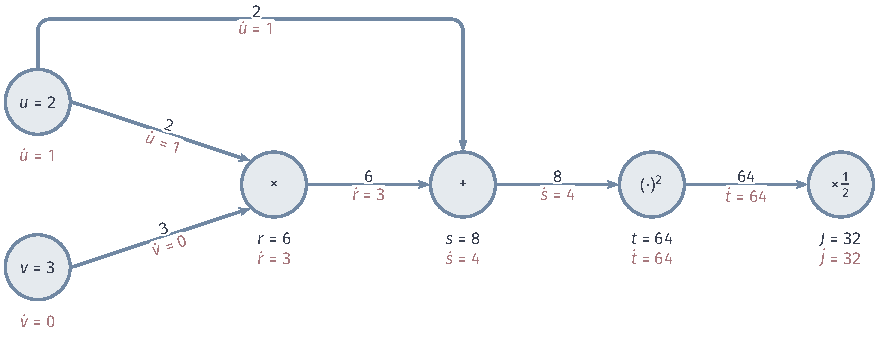
\includegraphics[width=148.791mm]{figures/05-neural-network-models/00-shared/tikz/ffn-autodiff-forward/figure.pdf}
  \caption{具体算子图上的前向模式。圆形节点表示乘法、加法、平方和缩放；实线上方的前向数字是传入算子的值，下方红色数字是同一路径上的方向导数。每个算子下方再用两行列出其输出值和输出方向导数。输入方向$(1,0)$给出$\partial J/\partial u=32$；加法处的$\dot s=3+1$包含了$u$的两条路径。}
  \label{fig:ffn-autodiff-forward}
\end{figure*}

图~\ref{fig:ffn-autodiff-forward}把一次方向导数计算附在原有算子图上。若要计算对$v$的偏导，改取$(\dot u,\dot v)=(0,1)$：此时$\dot r=2$、$\dot s=2$、$\dot t=32$，最终$\dot J=16$。两次遍历的前向值相同，变化的是输入方向以及随之传播的导数。

\FloatBarrier
\subsubsection{后向模式与梯度累加}
\label{sec:ffn-autodiff-reverse}

若希望从一个标量目标同时得到多个输入的导数，可以反过来问：输出对当前中间值有多敏感？\term{后向模式}（reverse mode）从输出向输入累积这种敏感度。记$\bar r=\partial J/\partial r$，对其他变量采用相同横线记号；前向值仍保留在原算子图中，从$\bar J=1$开始回传：
\begin{equation}
  \begin{aligned}
    \bar t&=\tfrac12\bar J,&\bar s&=2s\bar t,\\
    \bar r&=\bar s,&\bar u&=\bar r v+\bar s,\\
    &&\bar v&=\bar r u\text{。}
  \end{aligned}
  \label{eq:ffn-reverse-mode}
\end{equation}
每条回传贡献等于下游敏感度乘该条依赖的局部导数。缩放算子给出$\bar t=1/2$，平方算子利用保存的$s=8$得到$\bar s=8$，加法向两个输入各传递$8$。其中传给$r$的$8$再经过乘法，分别给$u$和$v$贡献$8v=24$与$8u=16$。

\begin{figure*}[htb]
  \centering
  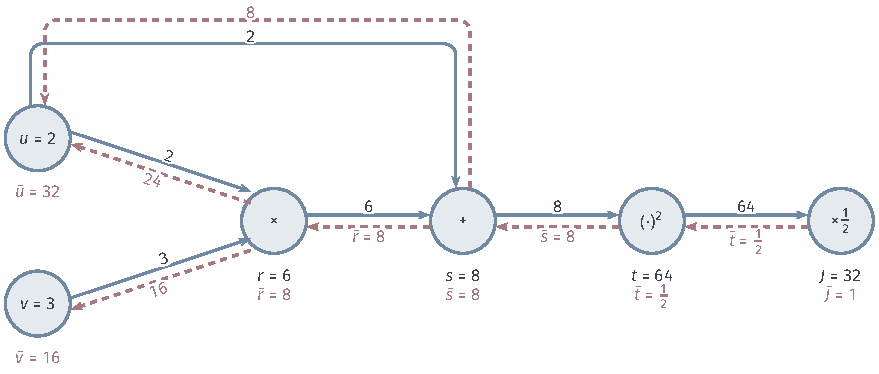
\includegraphics[width=148.791mm]{figures/05-neural-network-models/00-shared/tikz/ffn-autodiff-reverse/figure.pdf}
  \caption{同一算子图上的后向模式。节点位置与前向模式相同，实线及其前向标注保留前向传递值，红色虚线及其标注从$\bar J=1$开始回传导数贡献；每个算子下方两行分别给出输出值和伴随值。输入$u$收到经乘法传来的$24$和直接经加法传来的$8$，累加为$32$；输入$v$得到$16$。一次后向遍历同时得到两个偏导。}
  \label{fig:ffn-autodiff-reverse}
\end{figure*}

在图~\ref{fig:ffn-autodiff-reverse}中，$u$有两条通向目标的路径，所以$\bar u=24+8=32$。若漏掉直接进入加法的路径，就会错误地得到$24$。共享参数在多处被使用时也遵循同样规则：先保存各使用位置的局部回传贡献，再把它们累加到同一个参数。后向模式改变的是求导顺序，原函数的前向依赖并没有改变。

\FloatBarrier
\subsubsection{两种模式的计算代价}
\label{sec:ffn-autodiff-cost}

前面的算例有两个输入、一个输出。在$(u,v)=(2,3)$处，$J$的Jacobian矩阵是一行$(32,16)$：前向种子$(1,0)$取出第一列，前向种子$(0,1)$取出第二列；后向种子$\bar J=1$则把这一整行的转置作为输入梯度返回。一般映射可以有多个输出，这时后向模式也需要指定从哪些输出开始、各占多少权重。

对一般映射$\bm{F}:\mathbb{R}^{p}\to\mathbb{R}^{q}$，Jacobian矩阵$\bm{J}_{\bm{F}}\in\mathbb{R}^{q\times p}$的行对应输出坐标、列对应输入坐标，梯度采用列向量。前向模式在给定输入方向$\bm{v}\in\mathbb{R}^{p}$时计算$\bm{J}_{\bm{F}}\bm{v}$，后向模式在给定输出权重$\bm{u}\in\mathbb{R}^{q}$时计算$\bm{J}_{\bm{F}}^{\top}\bm{u}$。二者都可直接计算乘积，无需存储完整Jacobian矩阵。用逐坐标方向构造完整Jacobian矩阵时，前向模式需要$p$个方向，后向模式需要$q$个方向；实际代价还取决于批处理、稀疏结构和基本算子的实现。

把一般映射的输入写为$\bm\theta\in\mathbb R^p$，并固定一个与输入无关的输出权重$\bm u$。后向种子$\bm u$所指定的求导对象，是加权标量$\psi_{\bm u}(\bm\theta)=\bm u^{\top}\bm F(\bm\theta)$；对第$k$个输入坐标求导，有
\[
  \frac{\partial\psi_{\bm u}}{\partial\theta_k}
    =\sum_{i=1}^{q}u_i\frac{\partial F_i}{\partial\theta_k},
  \qquad
  \nabla_{\bm\theta}\psi_{\bm u}
    =\bm J_{\bm F}^{\top}\bm u\text{。}
\]
因此一次后向计算把各输出对输入的影响，按所选权重相加。取$\bm u$为第$i$个输出坐标的标准基向量，就只保留$F_i$，返回Jacobian第$i$行的转置。逐个选择全部$q$个输出坐标，才恢复全部行。

前向模式则把Jacobian的各列按输入方向的坐标加权，即
\[
  \bm J_{\bm F}\bm v=\sum_{k=1}^{p}v_k(\bm J_{\bm F})_{:,k}\text{。}
\]
取第$k$个输入标准基向量，就只保留第$k$列，逐个选择$p$个输入坐标才恢复全部列。前面标量算例正是$p=2$、$q=1$的情形；训练虽可输出多个类别得分，损失汇总后仍是一个标量，所以对参数求损失梯度只需一个后向种子$1$。

神经网络训练通常有很多参数，却只有一个标量目标，即$q=1$。后向模式从该目标出发，能够在与前向求值同阶的算术工作中得到完整参数梯度，代价是保存或重新计算反向所需的中间值。前述反向传播就是后向模式在神经网络损失上的具体应用\scite{baydin2018autodiff}

如果计算图包含多条损失分支，梯度在共同上游节点相加；如果某些分支被有意停止求导，它们就不再贡献上游梯度。离散采样、取整和按值选择分支也需要分别判断可微性：自动微分通常沿当前执行路径应用已登记的规则，不会自行补上对离散选择概率的导数。核验所得梯度时，需要同时检查目标、依赖路径和特殊算子的求导规则；数值梯度检查可进一步检验选定点附近的计算。

\section{前馈神经网络的扩展}
\label{sec:ffn-extensions}

前两节默认输入已经是一串数值。但真实数据里充满了\emph{类别信息}：设备型号、用户性别、语言中的词、商品编号。这些对象的共同特点是：它们用一个“编号”或“名字”标识身份，编号本身却不携带任何可以直接计算的数值含义——把“手机”编号成3并不意味着它是“平板（编号2）”的1.5倍。如果直接把编号当成一个实数喂给网络，模型就会被迫在编号的大小关系上做文章，而这种大小关系完全是人为随意指定的。

解决办法是把\emph{输入接口也纳入学习}：不让类别以一个编号数字进入，而是为每个类别学习一个简短的实数向量，让向量中各坐标的取值由任务数据决定；类别先经过这个可学习向量，再接入前面的前馈计算。这样，表示向量和后续预测参数就能由同一个任务共同调整。这一机制称为Embedding（嵌入），它不仅用于传统表格中的类别字段，也是现代语言模型处理词和符号的基础。

\subsection{支持高维离散表示：Embedding}
\label{sec:ffn-embedding}

考虑由设备类别和使用状态预测下一时间窗是否发生故障。使用时长等数值有单位和大小关系，设备类别的编号却只是身份标记。下面先用这项任务说明怎样为类别学习向量，再说明训练所得表示怎样预训练、迁移和部署使用。

\subsubsection{从高维稀疏表示到低维稠密表示}
\label{sec:ffn-embedding-motivation}

假设三个设备类别分别编号为$1,2,3$。若把编号直接作为一个实数送入线性单元，类别贡献就被写成$wc+b$，相邻编号之间的差别都由同一个$w$决定。重新给类别编号，还会改变这种数值关系。后续非线性网络可以学习更复杂的响应，但编号本身没有提供“类别2应处于类别1与类别3之间”的依据，因此不宜把身份编号的大小当成任务已知的规律。

一种不引入这种顺序的做法，是干脆不用一个数字、而是为每个类别单独分配一个坐标。编号为$c$的类别由向量$\bm{o}(c)$表示：第$c$个坐标为$1$，其他坐标为$0$。这就是\term{独热表示}（one-hot representation）。例如三个类别的向量分别为$(1,0,0)^{\top}$、$(0,1,0)^{\top}$和$(0,0,1)^{\top}$。它用“在哪个位置上为1”来表示身份，彻底去掉了编号之间的大小和顺序。其代价也很明显：任意两个不同类别之间的欧氏距离都等于$\sqrt{2}$，模型从表示本身得不到“哪两类更相近”的任何提示；哪些类别在当前任务中作用相近，必须由后续模型从数据中学习。

当类别很多时，独热向量的维度会随类别数增长。若直接接一个全连接层，每个类别还对应这一层的一整列权重。我们可以改为先给每个类别保存一个较短的可学习向量，让后续单元读取同一组向量坐标。这种把对象转成向量、供后续计算使用的表示称为\term{嵌入}（embedding）。这里具体学习的是类别身份到向量的映射，向量各坐标通常没有预先指定的名称，两个类别也可能得到相同向量。嵌入不是额外找回原始记录中的信息；它改变的是已知类别进入模型的参数化方式。

在类别数很大时，独热表示只有一个非零坐标，其余坐标都是零，因此是高维稀疏表示。本节关注嵌入宽度小于类别数的情形，将这种输入转换为较短的稠密向量：向量不再受“恰好一个坐标为$1$、其余为$0$”的限制，通常多个坐标同时取非零值。“稠密”并不要求每个坐标都非零，含有零坐标的向量也可以作为这类表示。这里的维度降低也不自动保证总参数更少，后面还需把嵌入表和后续投影一起计数。

\subsubsection{网络架构}
\label{sec:ffn-embedding-architecture}

设类别共有$K$个，类别编号$c\in\{1,\ldots,K\}$，嵌入宽度为$d_e$。用矩阵$\bm{E}\in\mathbb{R}^{K\times d_e}$保存参数，每一行存放一个类别的向量。为保持本章的列向量约定，取出第$c$行后将它转置，得到$\bm{e}_c\in\mathbb{R}^{d_e}$。这一操作也可以用独热向量写成
\begin{equation}
  \bm{e}_c=\bm{E}^{\top}\bm{o}(c),
  \qquad (\bm{e}_c)_k=E_{c,k},\quad k=1,\ldots,d_e\text{。}
  \label{eq:ffn-embedding-lookup}
\end{equation}
由于$\bm{o}(c)$只有一个非零坐标，乘法只选出对应的一行，并不需要真的生成长独热向量或执行完整稠密乘法。这种按编号读取参数向量的模块称为\term{嵌入层}（embedding layer）。单个编号的查表需要读取$d_e$个数，整张表仍需保存$Kd_e$个参数。独热输入上的线性映射与查表可以给出同一个结果，查表本身没有增加非线性。

回到故障预测，设$\bm{x}\in\mathbb{R}^{r}$记录预测时刻已经知道并按训练规则处理的数值变量。把它与$\bm{e}_c$拼接，便得到$r+d_e$维输入。一个含$m$个隐藏单元的二分类网络可以写为
\begin{equation}
  \begin{aligned}
    \bm{h}&=\sigma(\bm{W}_x\bm{x}+\bm{W}_e\bm{e}_c+\bm{b}),\\
    a&=\bm{w}_o^{\top}\bm{h}+b_o,\qquad p=s(a)\text{。}
  \end{aligned}
  \label{eq:ffn-embedding-classifier}
\end{equation}
其中$\bm{W}_x\in\mathbb{R}^{m\times r}$、$\bm{W}_e\in\mathbb{R}^{m\times d_e}$、$\bm{b},\bm{w}_o\in\mathbb{R}^{m}$，$b_o$为标量，$s$是前文的Sigmoid。$p$表示模型给出的故障概率。类别先决定查哪一行，取出的向量再与数值变量共同影响隐藏活动；整条前向路径没有环。多个类别字段可以分别设置嵌入表，再把各字段的向量与数值变量拼接，字段的含义和编号映射需要分别保存。

图~\ref{fig:ffn-embedding-architecture}把查表与后续网络接成一条前向路径。图中先放嵌入坐标、再放数值坐标，得到拼接向量$\bm{v}=[\bm{e}_c;\bm{x}]$；对应的全连接权重按$[\bm{W}_e\;\bm{W}_x]$排列，仍然得到式\eqref{eq:ffn-embedding-classifier}中的同一个加权和。两条输入路径在这里保留各自的坐标，拼接不等于把两个向量相加。

\begin{figure*}[htbp]
  \centering
  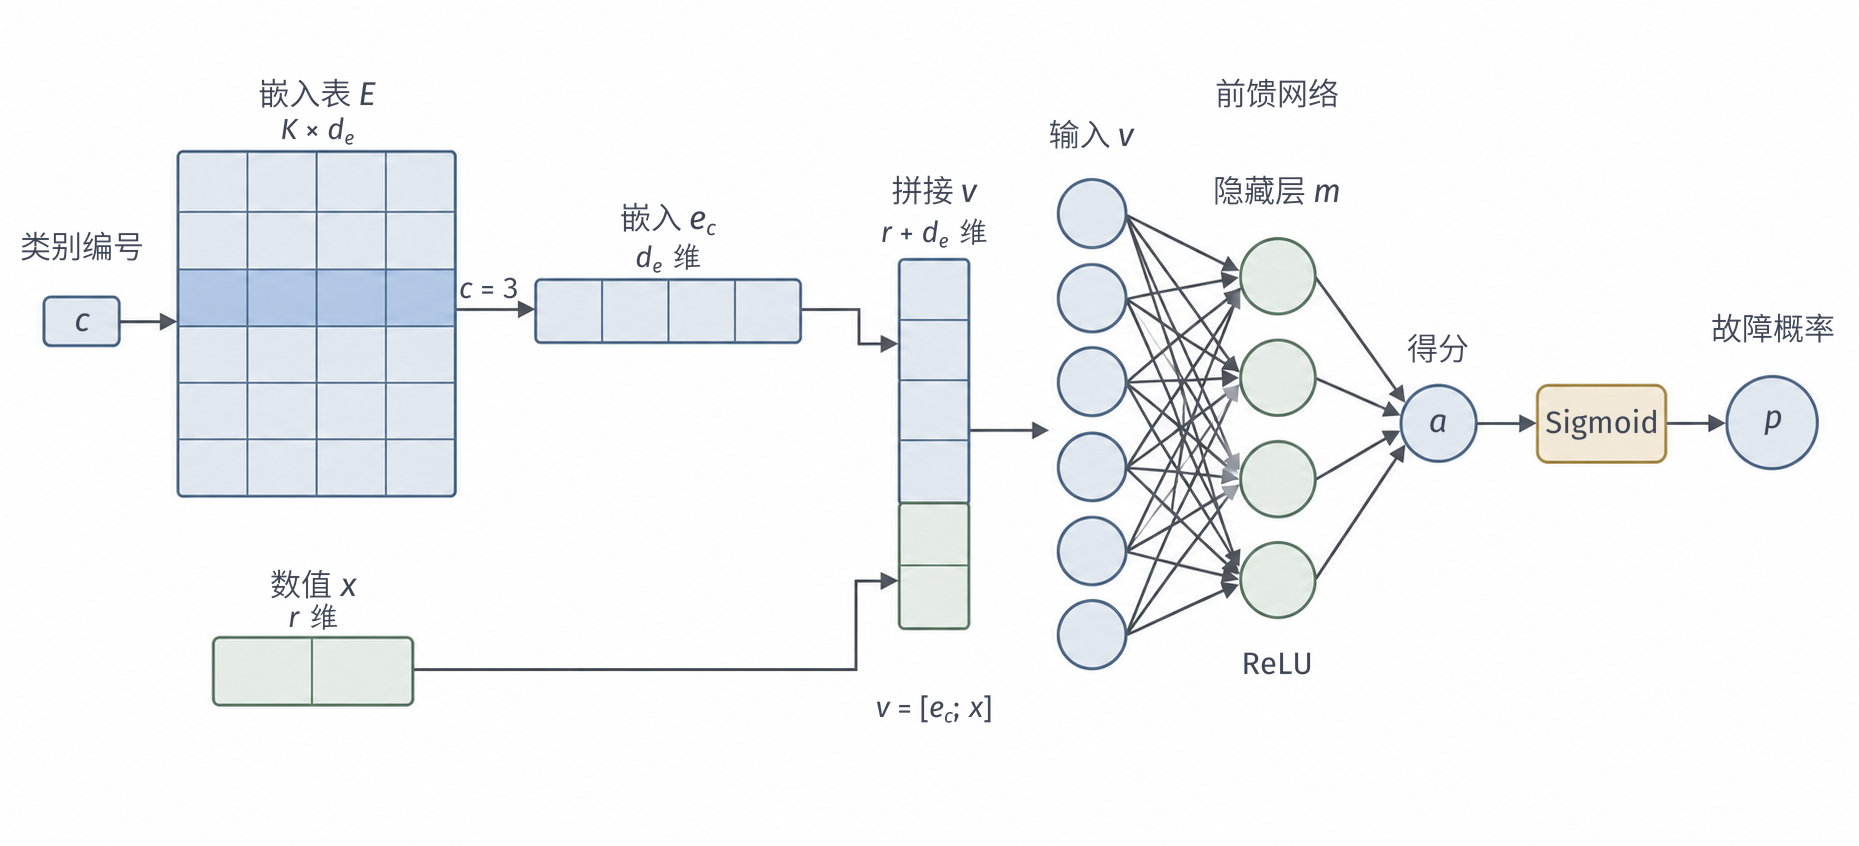
\includegraphics[width=169.000mm]{figures/05-neural-network-models/00-shared/generated/ffn-embedding-architecture/figure.png}
  \caption{嵌入层接入前馈二分类器的前向路径。教学示意取$K=6$、$d_e=4$、$r=2$、$m=4$，编号$c=3$选中嵌入表的第三行，读出四个嵌入坐标；横排的四格只表示坐标，数学运算仍采用列向量。蓝色嵌入与绿色数值特征按上四格、下两格拼接，右侧六个输入节点展开这六个坐标，经四个隐藏单元得到原始得分$a$，再经Sigmoid变成故障概率$p$。图只画前向计算，偏置未单独画出；格数和层宽是结构示意，不是训练实验。}
  \label{fig:ffn-embedding-architecture}
\end{figure*}
\FloatBarrier

较短向量引入了什么取舍，可以直接从第一层看出。若把独热向量直接送到同样宽度的隐藏层，类别部分需要一个$m\times K$矩阵。现在这部分变成$\bm{W}_e\bm{E}^{\top}$，参数数目由$mK$变为$Kd_e+md_e$，数值分支、偏置和输出层不参与这一比较。只有$d_e(K+m)<mK$时，这种分解才减少类别部分的参数；例如教学设定$K=100000$、$m=128$、$d_e=32$时，两者分别为$12800000$和$3204096$。查表避免生成独热向量，参数分解则在上述条件下减少存储，两项作用应分开判断。

这种分解也限制了类别到隐藏预激活的线性映射：$\bm{W}_e\bm{E}^{\top}$的秩至多为$d_e$，当$d_e<\min\{m,K\}$时，不能表达任意$m\times K$矩阵。不同类别仍有各自的一行参数，但后续计算共用$\bm{W}_e$对这$d_e$个坐标的解释。较小$d_e$可能提供适合任务的限制，也可能舍去任务需要的区别。因此，嵌入宽度是需要结合验证数据选择的超参数，不能由“使用了embedding”就推出表达更强、参数更少或预测更准确。

\FloatBarrier
\subsubsection{参数学习}
\label{sec:ffn-embedding-training}

向量的数值需要由数据确定。故障预测的一条训练记录为$(\bm{x}_i,c_i,y_i)$，其中$y_i\in\{0,1\}$说明指定时间窗内是否发生故障。用$\bm{\phi}$收集式\eqref{eq:ffn-embedding-classifier}中除嵌入表以外的网络参数，按前面的二元交叉熵比较预测与标签，可以共同学习$\bm{E}$和$\bm{\phi}$：
\begin{equation}
  \begin{aligned}
    \min_{\bm{E},\bm{\phi}}\quad &
    \frac{1}{n}\sum_{i=1}^{n}\ell(a_i,y_i)
    +\lambda\Omega(\bm{E},\bm{\phi}),\\
    \ell(a_i,y_i)&=\log(1+\exp(a_i))-y_i a_i\text{。}
  \end{aligned}
  \label{eq:ffn-embedding-objective}
\end{equation}
$a_i$由当前参数、$\bm{x}_i$和第$c_i$行嵌入计算得到，$\lambda\geq0$控制可选惩罚$\Omega$。这里奖励的是故障预测所需的表示，没有直接要求故障倾向相近的不同类别向量也具有较大的余弦相似度。不同坐标可以重新缩放，同时对下游权重作相反缩放而保持预测不变；这样的变化却可能改变向量夹角。因此，一个分类目标学到的嵌入不能自动解释成适合余弦检索的表示。

把这种缩放写成矩阵，可以区分统一倍乘与逐坐标改变尺度。令$\bm D$是对角元素均为正的可逆对角矩阵，把每个嵌入改为$\bm e'_c=\bm D\bm e_c$，同时把下游投影改为$\bm W'_e=\bm W_e\bm D^{-1}$。嵌入表相应变为$\bm E'=\bm E\bm D$，因为表中存放的是这些列向量的转置。于是$\bm W'_e\bm e'_c=\bm W_e\bm e_c$，其他参数不变时，隐藏预激活、预测概率和数据损失都保持不变。若不同坐标采用不同倍数，夹角却可能变化。例如$(1,1)^{\top}$与$(1,-1)^{\top}$原来的余弦为$0$；取$\bm D=\operatorname{diag}(2,1)$后，两向量变成$(2,1)^{\top}$与$(2,-1)^{\top}$，余弦为$(4-1)/(\sqrt5\sqrt5)=3/5$。这项等价只针对数据预测；参数惩罚$\Omega$可能随缩放改变，不能据此断言完整训练目标也不变。

反向传播怎样经过查表，可以从当前样本的损失开始。令$\bm{z}_i=\bm{W}_x\bm{x}_i+\bm{W}_e\bm{e}_{c_i}+\bm{b}$。在激活可微处，或采用前文约定的分段求导规则时，损失对嵌入向量的梯度为
\begin{equation}
  \bm{g}_i=\nabla_{\bm{e}_{c_i}}\ell
  =\bm{W}_e^{\top}\left[
    (p_i-y_i)\bm{w}_o\odot\sigma'(\bm{z}_i)
  \right]\in\mathbb{R}^{d_e}\text{。}
  \label{eq:ffn-embedding-vector-gradient}
\end{equation}
这仍是本章已经推导的链式法则：输出的$p_i-y_i$先传到隐藏层，再经过$\bm{W}_e$传到嵌入坐标。对表中元素$E_{c,k}$求导时，只有$c=c_i$才会经过这次读取，且该行第$k$项的局部导数为$1$。因此，小批量$B$的数据损失对整张表的梯度为
\begin{equation}
  \nabla_{\bm{E}}\frac{1}{|B|}\sum_{i\in B}\ell(a_i,y_i)
  =\frac{1}{|B|}\sum_{i\in B}\bm{o}(c_i)\bm{g}_i^{\top}\text{。}
  \label{eq:ffn-embedding-table-gradient}
\end{equation}
外积的形状为$K\times d_e$，每个样本把梯度放到自己读取的行；同一类别在批内多次出现时，贡献加到同一行。编号$c_i$是固定的离散选择，不需要对编号本身求导，待学习的是选中行的实数参数。这解释了为什么查表能够参加反向传播，而不是要求类别编号也连续可微。

\begin{example}[一次嵌入查表与更新]
  \label{ex:ffn-embedding-update}
  取三个设备类别、二维嵌入和两个ReLU隐藏单元，以下数值只是教学构造：
  \[
    \begin{aligned}
      \bm{E}&=\begin{pmatrix}1&0\\0&1\\1&1\end{pmatrix},
      &\bm{W}_x&=\begin{pmatrix}1\\-1\end{pmatrix},\\
      \bm{W}_e&=\bm{I}_2,
      &\bm{b}&=\bm{0},\\
      \bm{w}_o&=\begin{pmatrix}1\\-1\end{pmatrix},
      &b_o&=0\text{。}
    \end{aligned}
  \]
  令数值输入为$x=0.5$，类别为$c=3$，标签为$y=1$。查表得到$\bm{e}_3=(1,1)^{\top}$，因此$\bm{z}=(1.5,0.5)^{\top}$，两个ReLU都处于正半轴，$\bm{h}=\bm{z}$。输出为$a=1$、$p=s(1)\approx0.7311$，交叉熵约为$0.3133$。

  式\eqref{eq:ffn-embedding-vector-gradient}给出$\bm{g}\approx(-0.2689,0.2689)^{\top}$。若不加惩罚，学习率取$0.1$，普通梯度下降使第3行对应的列向量变为
  \[
    \bm{e}_3^{\mathrm{new}}
    =\bm{e}_3-0.1\bm{g}
    \approx(1.0269,0.9731)^{\top}\text{。}
  \]
  这一行的两个坐标沿不同方向调整，是因为当前输出用第一坐标减第二坐标来预测正类。前两行没有来自这次查表的数据梯度。这里单独展示表参数的变化；联合训练时，其余网络参数也按同一更新前参数计算梯度，再一起更新。
\end{example}

实际训练可以从适当尺度的随机嵌入表开始，其他层按前面与激活相配的规则初始化，然后沿算法~\ref{alg:ffn-minibatch-learning}执行查表、前向、反向和小批量更新，并按验证指标选择停止时刻与参数。若加入全表惩罚、使用带历史状态的优化器，或让这张表还参加输出计算，未在当前输入中查到的行也可能得到其他梯度或更新；上面“只进入选中行”的结论仅针对这次查表路径的数据梯度。少见类别的行得到的直接训练信号较少，单独保留一行参数也不能保证新类别有可靠表示。

\subsubsection{表达的使用}
\label{sec:ffn-embedding-use}

训练得到的嵌入首先要按训练时的接口使用。部署时需要连同参数保存类别到行号的映射和数值变量的转换规则：新记录先作相同预处理，再映射编号、查表、按式\eqref{eq:ffn-embedding-classifier}计算输出，分类任务按验证阶段确定的阈值决策。若重新排列类别编号却没有同步排列嵌入表，即使表内数值不变，也会把错误类别的向量交给网络。未见类别不能靠随机增加一行获得含义：可让多个未登记类别共用一个经过训练的未知项，舍去它们之间的区别；也可利用属性或文本描述经另一个表示网络计算向量，但这需要可获得的属性和相应训练依据。稀有类别得到的直接信号少，大表的存储仍按$Kd_e$增长，都要单独评价。

当前任务标签较少时，表示可以先在数据更多的其他目标上\emph{预训练}（pretraining）再迁移，但前提是两个任务共享可对应的输入：同一套设备编号可以复用对应行，词元表与设备编号之间没有行对应，就不能直接互换。一种不依赖人工类别的目标是词元预测：对固定窗口内的词元查表，接前馈网络用Softmax预测下一个词元，目标由文本自身构造，同一词元在不同窗口的梯度累加到同一行；这样学到的是服务于词元预测的表示，不自动适合故障分类或检索\scite{goodfellow2016}。若预期用途是检索，还需把“应当找回哪个对象”写进目标：设查询$\bm{u}$与$M$个候选文档向量$\bm{v}_j$均按式\eqref{eq:ffn-normalized-representation}归一化，以匹配文档为正确类，用温度$\tau>0$缩放余弦相似度后作候选Softmax，
\begin{equation}
  \ell_{\mathrm{pair}}
  =-\log\frac{\exp(\bm{u}^{\top}\bm{v}_1/\tau)}
  {\sum_{j=1}^{M}\exp(\bm{u}^{\top}\bm{v}_j/\tau)}\text{。}
  \label{eq:ffn-embedding-contrastive}
\end{equation}
这就是\term{对比学习}（contrastive learning）的一种形式：它沿用多类交叉熵，奖励匹配分数相对不匹配候选提高；若所有向量相同，损失为$\log M$，没有区分作用。负例选择和多个匹配文档的处理都要按任务规定；词元预测、故障分类与文档匹配给出的约束不同，学到的邻域关系也不必相同。这里的查询—文档训练组是教学构造，并非所引视觉对比方法的图像增强流程\scite{chen2020}

迁移到新任务时有两种参数选择。\emph{冻结}（freeze）表示保留嵌入表或编码器、只训练新任务的输出头，需要更新的参数少，但不能修正不合适的表示；\emph{微调}（fine-tuning）允许新任务损失继续更新表示，适应能力更强，但需要足够的当前数据支撑。两者都必须使用与预训练匹配的词表、切分、维度和预处理，并在当前任务的验证集上比较，不能只凭向量看起来成簇判断收益。检索场景还要先保存文档向量，查询到来时只编码查询、按约定的归一化与相似度排序返回；编码器或输入规则更新后，已保存的向量要重新计算，不同训练版本的同维向量不能仅凭维度相同混用。

最后区分查表向量与上下文表示。嵌入表对同一编号总返回同一向量，与它本次出现在什么句子中无关；要区分同一词在不同语境中的用法，后续网络必须读取上下文再计算表示。对多个词元取平均会丢失顺序，按固定位置拼接则保留窗口内的位置信息。因此embedding既可以是输入端的可学习查表，也可以是编码器输出的对象向量；其可用含义由输入、训练目标和实际使用方式共同决定。

\section{理论分析}
\label{sec:ffn-theory}

到目前为止，本章回答的都是“网络怎么算、怎么训”的操作性问题。本节退一步，回答三个决定这套方法是否可信的理论问题，它们恰好对应训练一个网络时最容易被混为一谈的三个阶段：
\begin{itemize}
  \item \emph{表达能力}：在所有可能的参数取值中，网络\textbf{能不能}表示（或足够逼近）我们想要的那个函数？这是“候选集合里有没有好答案”的问题，与训练无关。
  \item \emph{收敛性}：即使好参数确实存在，梯度下降\textbf{能不能}找到它，或者至少走到梯度足够小的点？这是“搜索算法找不找得到”的问题。
  \item \emph{泛化性}：即使在训练集上找到了损失很低的参数，它在没见过的新样本上\textbf{风险有多大}？这是“找到的答案能不能推广”的问题。
\end{itemize}
这三个问题需要分别判断，对其中一个的肯定回答不能代替另外两个：网络可以表达一切连续函数却难以优化，可以在训练集上损失为零却对新样本频频出错。下面三小节依次展开，并始终标明每个结论成立所需要的条件。

\subsection{表达能力}
\label{sec:ffn-expressivity}

先问最基本的存在性问题：给定一个想要学习的函数（比如一条复杂的非线性曲线），神经网络的参数空间里到底\emph{存不存在}一组参数能把它表示出来？前章的异或例子是一个精确表示结论：在指定的四个输入点上，确实存在一组参数使输出与标签完全一致。但真实输入通常是连续的，目标函数也往往不是四个离散点，这时更常见的问题是：能否让网络与目标函数\emph{足够接近}（误差小于任意给定的小正数$\varepsilon$），而不必逐点精确相等。\term{表达性}（expressivity）描述的就是网络族能够表示或逼近哪些函数；注意它的判断对象是\emph{整类}可选参数所形成的函数集合，而不是某次训练实际得到的那一个网络。

\begin{theorem}[前馈网络对紧集上连续目标的逼近能力]
\label{thm:ffn-continuous-approximation}
设$D\subset\mathbb R^d$为非空紧集，目标$g:D\to\mathbb R^q$连续。激活函数连续且不是多项式，网络允许隐藏偏置和线性输出。对任意$\varepsilon>0$，存在有限宽度的单隐藏层网络$f$，使
\[
 \sup_{\bm x\in D}\lVert f(\bm x)-g(\bm x)\rVert_2<\varepsilon\text{。}
\]
因此，对任意支撑在$D$上的输入分布$P_X$，同一候选满足
$\lVert f-g\rVert_{L^2(P_X)}<\varepsilon$。
\end{theorem}
标量情形见\BookChapterRef{chap:functional-analysis-and-approximation}{卷1《数学准备：计算、分析与几何》的“函数空间”章}；向量目标可逐坐标逼近：给每个坐标分配$\varepsilon/\sqrt q$的误差，把各标量网络的隐藏单元并列放入同一隐藏层、让第$j$个线性输出只读取自己那组单元，就得到有限宽度的向量网络。由于$P_X$是支撑在$D$上、总质量为一的概率测度，一致误差小于$\varepsilon$也控制$L^2(P_X)$平均误差。这里的宽度和参数可以随目标及精度改变，固定规模不享有任意精度保证；对分类问题可逐坐标逼近连续的条件概率函数，不连续目标或不受限输入域则需要另外分析。

通用逼近定理回答了“只要足够宽就能逼近”，但“宽”和“深”是两种不同的增加复杂度的方式：前者是在同一层并排更多单元，后者是把已有变换反复复合。要理解深度的独特作用，最好看一个函数，它用深网络表示很省、用浅网络表示却需要指数级数量的单元。

ReLU网络的一个直接读法是分段仿射变换。在一组隐藏单元的正负状态固定的输入区域内，每个ReLU都等价于原样保留某坐标或置零，整个网络因而是仿射的；不同的正负状态组合形成不同区域。有限个区域拼接起来就能近似弯曲形状，而一个固定大小的网络只有有限个这种区域。

一维情形能把这种拼接写成明确公式。设连续分段线性函数的内部转折点为$t_1<\cdots<t_m$，从左到右的斜率为$s_0,s_1,\ldots,s_m$，则可写成
\begin{equation}
  f(x)=c+s_0x+
  \sum_{j=1}^{m}(s_j-s_{j-1})\rho(x-t_j)\text{。}
  \label{eq:ffn-piecewise-linear-representation}
\end{equation}
每个ReLU项在对应转折点之后改变斜率，相邻段斜率在求和中逐项抵消，恰为当前段的$s_k$；$c$对齐整体高度，若网络没有直接的线性输入支路，可用$x=\rho(x)-\rho(-x)$补出$s_0x$。因此增加宽度就是增加可表达的转折。另一方面，紧区间上的连续函数由一致连续性，可取足够密的节点作线性插值，使节点间误差任意小；这条折线再由上式表示，就给出一维ReLU网络通用逼近的构造直觉。

深度提供另一种组织复杂函数的方式：重复复用已有变换。考虑$[0,1]$上的三角形函数
\begin{equation}
  T(x)=2\rho(x)-4\rho(x-1/2)+2\rho(x-1)\text{。}
  \label{eq:ffn-tent-function}
\end{equation}
它在$[0,1/2]$从$0$上升到$1$，在$[1/2,1]$再下降到$0$。令$T_k$表示$T$复合$k$次，而不是$T$的$k$次幂。每复合一次，每个线性区间又被分成两段，归纳可得$T_k$在$[0,1]$上有$2^k$个线性区间。

\begin{figure*}[htb]
  \centering
  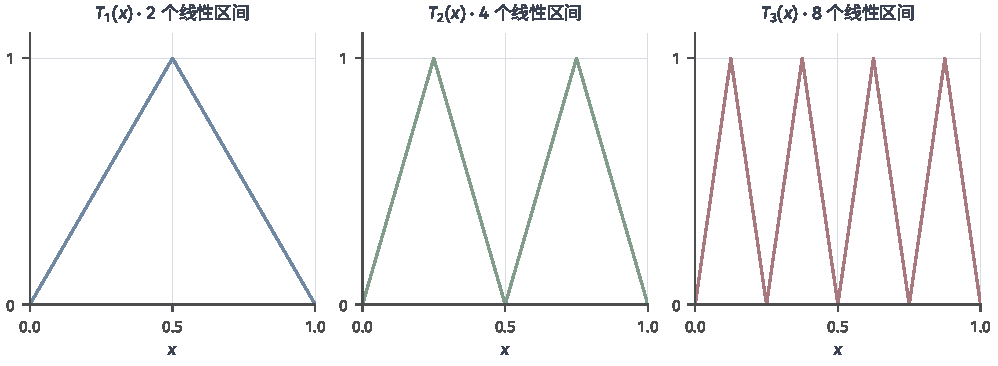
\includegraphics[width=159.059mm]{figures/05-neural-network-models/00-shared/matplotlib/ffn-depth-composition/figure.pdf}
  \caption{三角形函数的复合产生更多转折。三幅解析图分别为$T_1=T$、$T_2=T\circ T$和$T_3=T\circ T\circ T$，横轴均为$x\in[0,1]$，纵轴为函数值。每次复合将线性区间数翻倍；这是一维构造，不是实际训练实验，也不表示任意目标都能从增加深度中获得相同收益。}
  \label{fig:ffn-depth-composition}
\end{figure*}

这一复合可以落实为宽度固定的串联MLP：每个阶段只需三个隐藏单元读出$\rho(u)$、$\rho(u-\tfrac12)$、$\rho(u-1)$，再按系数$(2,-4,2)$线性组合并补上相应偏置，就得到下一阶段的输入$u$；重复$k$个这样的宽度为$3$的阶段、末端接线性读出即可，相邻阶段间的仿射映射可并入下一层权重。另一方面，$T_k$相邻段的斜率正负交替，$2^k$段之间确有$2^k-1$个不能合并的内部转折；而单隐藏层的一维ReLU网络中每个单元至多引入一个转折，精确表示$T_k$至少需要$2^k-1$个隐藏单元。图~\ref{fig:ffn-depth-composition}展示了这种重复组合的效率：深度随$k$线性增长、宽度保持常数，浅层表示却需要指数级单元。更一般的深度分离结果还需固定误差度量、目标函数族和比较网络的范围\scite{telgarsky2016depth}

这个例子固定同一个三角形复合目标，比较浅层与深层表示所需的单元数；训练难度和新样本风险是另外两个评价对象。某些目标用浅层结构已经足够；若目标本身具有可复用的组合规律，深度才可能以较少单元组织这种规律。表达能力的分析因此应同时说明目标、激活、深度、宽度和逼近精度。


\subsection{收敛性}
\label{sec:ffn-convergence}

隐藏层与输出层共同学习时，参数通过多层复合相互耦合，训练目标通常非凸。对于有下界、梯度为$\beta$-Lipschitz的光滑目标，完整梯度下降采用不超过$1/\beta$的固定正步长，可以使前若干步的平均平方梯度随步数增加而趋于零。这保证迭代中出现接近一阶驻点的位置，不能保证到达全局最优；ReLU拐点、小批量抽样和自适应更新还需各自的条件。相关优化结论可参考\BookChapterRef{chap:optimization}{卷1《数学准备：计算、分析与几何》的“最优化”章}。

固定隐藏表示、只学习带正二次惩罚的线性回归读出时，目标成为严格凸二次问题，具有唯一解；端到端训练通常不具备这份凸性。反向传播负责正确计算学习信号，优化器和停止规则怎样使用它，可参考本卷第\ref{chap:neural-network-training}章。

\subsection{泛化性}
\label{sec:ffn-learnability}

训练误差低还需要与有限样本的泛化保证一起判断。在独立同分布抽样、输入与损失满足相应尺度条件时，候选函数的复杂度或学习算法的稳定性可以控制训练风险与新样本期望风险的差距。对分类网络，参数范数还要与分类间隔一起考察；仅增加宽度或减小某一层权重，均不能单独保证预测更可靠。相关结论可参考\BookChapterRef{chap:deep-learning-theory}{卷3《基础、理论与可信性》的“深度学习的可学习性”章}。

合适的表示、充分且独立的样本，以及有效的训练共同决定新样本误差。训练与部署的分布不同，或多条记录来自同一对象而相互依赖时，还需按实际数据条件评价。本卷第\ref{chap:neural-network-generalization}章进一步说明数据增强、正则化和训练选择的作用。

\section{本章小结}
\label{sec:ffn-summary}

前馈神经网络把可学习表示落实为一条没有有向环的计算路径。全连接层组合已有坐标，非线性激活让多层复合超出仿射映射，输出变换与损失共同规定训练所要预测的对象。选择层宽和激活时，既要看能够形成怎样的函数，也要看参数量、计算量和梯度传播条件。

隐藏层的学习信号来自最终目标对它的敏感度。反向传播按链式法则逐层汇总这种影响，用局部导数和已有活动值计算所有参数梯度；自动微分将同样的原则推广到程序的实际计算路径。初始化决定起点，优化器使用梯度作出更新，二者都影响学习结果，正确求导只是完成训练的一个条件。

Embedding把输入表示也纳入这一学习过程：类别编号选取一行参数，下游损失决定该行怎样变化；更一般的编码器则根据输入计算对象向量。训练目标决定向量需要保留什么，部署时的编号、输入处理和比较规则决定这些向量能否被正确复用。

表达能力说明网络中是否存在合适的函数，优化分析说明训练能够找到怎样的参数，泛化结论则需要样本与学习条件。这些判断不能互相替代。前馈网络适合处理定长数值表示；具有空间、序列或关系结构的数据，还需要下一章起介绍的相应连接方式。

\paragraph{扩展阅读}
Goodfellow等教材第6章展开前馈网络与反向传播，计算图中的共享依赖解释了各梯度为何累加；第8章讨论所得梯度怎样用于优化，第7章讨论正则化如何限制候选和影响学习结果。这些内容分别对应本章的计算、求解与泛化问题\scite{goodfellow2016}
